
\chapter{Stability of defection, optimisation of strategies and the limits of
       memory in the Prisoner's Dilemma.}\label{chapter:memory_one}

\begin{center}
    The research reported in this Chapter has lead in a manuscript, entitled: \\
    \textbf{``Stability of defection, optimisation of strategies and the limits of memory in the Prisoner's Dilemma''} \\
    Available at: \url{arxiv.org/abs/1911.12112} \\
    Associated data set: \cite{glynatsi2019} \\
    Axerod-Python library version: 4.4.0 \\ \vspace{.5cm}
    The manuscript's abstract is the following:
\end{center}

Memory-one strategies are a set of Iterated Prisoner's Dilemma strategies that
have been acclaimed for their mathematical tractability and performance against
single opponents. This manuscript investigates best responses to a collection of
memory-one strategies as a multidimensional optimisation problem. Though
extortionate memory-one strategies have gained much attention, we demonstrate
that best response memory-one strategies do not behave in an extortionate way,
and moreover, for memory one strategies to be evolutionary robust they need to
be able to behave in a forgiving way. We also provide evidence that memory-one
strategies suffer from their limited memory in multi agent interactions and can
be out performed by longer memory strategies.

The differences between the Chapter and the manuscript include \dots.

\newpage

\section{Introduction}\label{section:mem_one_introduction}

This Chapter contributes to the question: what is the optimal behaviour an
IPD strategy should adapt as a response to different environments? The environment
considered in this Chapter are against memory-one strategies.
In~\cite{Press2012} the authors stated that ``Only a player with a theory of
mind about his opponent can do better, in which case Iterated Prisoner's Dilemma
is an Ultimatum Game''. The purpose of this Chapter is to investigate the first
part of this sentence, more specifically, to investigate the best response
strategy with a theory of mind in an environment with memory-one opponents, and
to understand the effects of extortion and restricted memory in those
environments.

The outcomes of this Chapter reinforce known results which were presented in
Chapter~\ref{chapter:literature_review}. Namely that memory-one strategies must
be forgiving to be evolutionarily stable~\cite{Stewart2013, Stewart2016} and
that longer-memory strategies have a certain form of advantage over short memory
strategies~\cite{Hilbe2017, Pan2015}. The Chapter is structured as follows:

\begin{itemize}
    \item section~\ref{section:utility}, presents a closed form algebraic expression for
    the utility of a memory-one strategy to a given group of opponents.
    \item section~\ref{section:best_response_mem_one}, defines a compact method
    of identifying the best response memory-one strategy against a given set
    of opponents.
    \item section~\ref{section:reactive_strategies}, defines best response reactive
    strategies and demonstrate the usage of resultant theory in explicitly finding
    a reactive best response.
    \item section~\ref{section:numerical_experiments}, presents a series of numerical experiments
    and a well designed framework that allows the
    comparison of an optimal memory one strategy and a more complex strategy which
    has a larger memory.
    \item section~\ref{section:stability_of_defection}, presents a compact method of identifying environments
    for which cooperation in known to not occur.
\end{itemize}


\section{The Utility}\label{section:utility}

One specific advantage of memory-one strategies is their mathematical
tractability. They can be represented completely as an element of \(\R^{4}_{[0, 1]}\).
As previously discussed in Chapter~\ref{chapter:literature_review}, 
if a strategy is concerned with only the outcome of a single turn then there are
four possible `states' the strategy could be in;

\begin{itemize}
    \item both players cooperated, denoted as \(CC\)
    \item first players cooperated whilst the second player defected, denoted as \(CD\)
    \item first players defected whilst the second player cooperated, denoted as \(DC\)
    \item both players defected, denoted as \(DD\)
\end{itemize}

Therefore, a memory-one strategy can be denoted by the probability vector of
cooperating after each of these states; \(p=(p_1, p_2, p_3, p_4) \in \R_{[0,1]}
^ 4\).

In~\cite{Nowak1989} it was shown that it is not necessary to simulate the play
of a strategy $p$ against a memory-one opponent $q$. Rather this exact behaviour
can be modelled as a stochastic process, and more specifically as a Markov chain
(Figure~\ref{fig:markov_chain}) whose corresponding transition matrix \(M\) is
given by (\ref{eq:transition_matrix}). The long run steady state probability
vector \(v\), which is the solution to \(v M = v\), can be
combined with the payoff matrices of (\ref{eq:pd_definition}) to give the expected
payoffs for each player. More specifically, the utility for a memory-one
strategy \(p\) against an opponent \(q\), denoted as \(u_q(p)\), is given by
(\ref{eq:press_dyson_utility}).

\begin{figure}
    \centering
    \includestandalone[width=.35\textwidth]{src/chapters/05/tex/markov_chain}
    \caption{Markov Chain}
    \label{fig:markov_chain}
\end{figure}

\begin{equation}\label{eq:transition_matrix}
    M = \left[\begin{matrix}p_{1} q_{1} & p_{1} \left(- q_{1} + 1\right) & q_{1} \left(- p_{1} + 1\right) & \left(- p_{1} + 1\right) \left(- q_{1} + 1\right)\\p_{2} q_{3} & p_{2} \left(- q_{3} + 1\right) & q_{3} \left(- p_{2} + 1\right) & \left(- p_{2} + 1\right) \left(- q_{3} + 1\right)\\p_{3} q_{2} & p_{3} \left(- q_{2} + 1\right) & q_{2} \left(- p_{3} + 1\right) & \left(- p_{3} + 1\right) \left(- q_{2} + 1\right)\\p_{4} q_{4} & p_{4} \left(- q_{4} + 1\right) & q_{4} \left(- p_{4} + 1\right) & \left(- p_{4} + 1\right) \left(- q_{4} + 1\right)\end{matrix}\right]
\end{equation}


\begin{equation}\label{eq:press_dyson_utility}
    u_q(p) = v \cdot (R, S, T, P).
\end{equation}

This thesis has explored the form of \(u_q(p)\), to the author's knowledge no
previous work has done this, and it proves that \(u_q(p)\) is given by a ratio
of two quadratic forms~\cite{kepner2011}, Theorem~\ref{theorem:quadratic_form_u}.

\begin{theorem}\label{theorem:quadratic_form_u}
    The expected utility of a memory-one strategy \(p\in\mathbb{R}_{[0,1]}^4\)
    against a memory-one opponent \(q\in\mathbb{R}_{[0,1]}^4\), denoted
    as \(u_q(p)\), can be written as a ratio of two quadratic forms:

    \begin{equation}\label{eq:optimisation_quadratic}
    u_q(p) = \frac{\frac{1}{2}pQp^T + cp + a}
                {\frac{1}{2}p\bar{Q}p^T + \bar{c}p + \bar{a}},
    \end{equation}
    where \(Q, \bar{Q}\) \(\in \R^{4\times4}\) are square matrices defined by the
    transition probabilities of the opponent \(q_1, q_2, q_3, q_4\) as follows:

    \begin{center}
    \begin{equation}
    \resizebox{0.9\linewidth}{!}{\arraycolsep=2.5pt%
    \boldmath\(
    Q = \left[\begin{matrix}0 & - \left(q_{1} - q_{3}\right) \left(q_{2} - 5 q_{4} - 1\right) & q_{3} \left(q_{1} - q_{2}\right) & - 5 q_{3} \left(q_{1} - q_{4}\right)\\- \left(q_{1} - q_{3}\right) \left(q_{2} - 5 q_{4} - 1\right) & 0 & \left(q_{2} - q_{3}\right) \left(q_{1} - 3 q_{4} - 1\right) & \left(q_{3} - q_{4}\right) \left(5 q_{1} - 3 q_{2} - 2\right)\\q_{3} \left(q_{1} - q_{2}\right) & \left(q_{2} - q_{3}\right) \left(q_{1} - 3 q_{4} - 1\right) & 0 & 3 q_{3} \left(q_{2} - q_{4}\right)\\- 5 q_{3} \left(q_{1} - q_{4}\right) & \left(q_{3} - q_{4}\right) \left(5 q_{1} - 3 q_{2} - 2\right) & 3 q_{3} \left(q_{2} - q_{4}\right) & 0\end{matrix}\right]\)},
    \end{equation}
    \begin{equation}\label{eq:q_bar_matrix}
    \resizebox{0.8\linewidth}{!}{\arraycolsep=2.5pt%
    \boldmath\(
    \bar{Q} =  \left[\begin{matrix}0 & - \left(q_{1} - q_{3}\right) \left(q_{2} - q_{4} - 1\right) & \left(q_{1} - q_{2}\right) \left(q_{3} - q_{4}\right) & \left(q_{1} - q_{4}\right) \left(q_{2} - q_{3} - 1\right)\\- \left(q_{1} - q_{3}\right) \left(q_{2} - q_{4} - 1\right) & 0 & \left(q_{2} - q_{3}\right) \left(q_{1} - q_{4} - 1\right) & \left(q_{1} - q_{2}\right) \left(q_{3} - q_{4}\right)\\\left(q_{1} - q_{2}\right) \left(q_{3} - q_{4}\right) & \left(q_{2} - q_{3}\right) \left(q_{1} - q_{4} - 1\right) & 0 & - \left(q_{2} - q_{4}\right) \left(q_{1} - q_{3} - 1\right)\\\left(q_{1} - q_{4}\right) \left(q_{2} - q_{3} - 1\right) & \left(q_{1} - q_{2}\right) \left(q_{3} - q_{4}\right) & - \left(q_{2} - q_{4}\right) \left(q_{1} - q_{3} - 1\right) & 0\end{matrix}\right]\)}.
    \end{equation}
    \end{center}

    \(c \text{ and } \bar{c}\) \(\in \R^{4 \times 1}\) are similarly defined by:

    \begin{equation}\label{eq:q_matrix_numerator}
    \resizebox{0.3\linewidth}{!}{\arraycolsep=2.5pt%
    \boldmath\(c = \left[\begin{matrix}q_{1} \left(q_{2} - 5 q_{4} - 1\right)\\- \left(q_{3} - 1\right) \left(q_{2} - 5 q_{4} - 1\right)\\- q_{1} q_{2} + q_{2} q_{3} + 3 q_{2} q_{4} + q_{2} - q_{3}\\5 q_{1} q_{4} - 3 q_{2} q_{4} - 5 q_{3} q_{4} + 5 q_{3} - 2 q_{4}\end{matrix}\right]\),}
    \end{equation}
    \begin{equation}\label{eq:q_matrix_denominator}
    \resizebox{0.3\linewidth}{!}{\arraycolsep=2.5pt%
    \boldmath\(\bar{c} = \left[\begin{matrix}q_{1} \left(q_{2} - q_{4} - 1\right)\\- \left(q_{3} - 1\right) \left(q_{2} - q_{4} - 1\right)\\- q_{1} q_{2} + q_{2} q_{3} + q_{2} - q_{3} + q_{4}\\q_{1} q_{4} - q_{2} - q_{3} q_{4} + q_{3} - q_{4} + 1\end{matrix}\right]\),
    }
    \end{equation}
    and the constant terms \(a, \bar{a}\) are defined as \(a = - q_{2} + 5 q_{4} + 1\) and
    \(\bar{a} = - q_{2} + q_{4} + 1\).
\end{theorem}

\begin{proof}

It was discussed that \(u_q(p)\) it is the product of the steady state
vector \(v\) and the PD payoffs,

\[u_q(p) = v \cdot (R, S, T, P).\]

The dot product of \(v \cdot (R, S, T, P)\) gives,

\begingroup
\scriptsize
\begin{equation*}
    \resizebox{0.91\hsize}{!}{
    $u_q(p) = \left(
    \frac
        {\parbox{6in}{$ - p_{1} p_{2} (q_{1} - q_{3}) (P q_{2} - P - T q_{4}) + p_{1} p_{3} (q_{1} - q_{2}) (P q_{3} - S q_{4}) + p_{1} p_{4} (q_{1} - q_{4}) (S q_{2} - S - T q_{3}) + p_{2} p_{3} (q_{2} - q_{3}) (P q_{1} - P - R q_{4}) - $ \\
        $ p_{2} p_{4} (q_{3} - q_{4}) (R q_{2} - R - T q_{1} + T) + p_{3} p_{4} (q_{2} - q_{4}) (R q_{3} - S q_{1} + S) + p_{1} q_{1} (P q_{2} - P - T q_{4}) - p_{2} (q_{3} - 1) (P q_{2} - P - T q_{4}) + $ \\
        $ p_{3} (- P q_{1} q_{2} + P q_{2} q_{3} + P q_{2} - P q_{3} + R q_{2} q_{4} - S q_{2} q_{4} + S q_{4}) + p_{4} (- R q_{2} q_{4} + R q_{4} + S q_{2} q_{4} - S q_{2} - S q_{4} + S ) $ \\
        \hspace*{5cm} $ T q_{1} q_{4} - T q_{3} q_{4} + T q_{3} - T q_{4} - P q_{2} + P + T q_{4}$
        }}
        {\parbox{6in}{$
        p_{1} p_{2} (q_{1} q_{2} - q_{1} q_{4} - q_{1} - q_{2} q_{3} + q_{3} q_{4} + q_{3}) + p_{1} p_{3} (- q_{1} q_{3} + q_{1} q_{4} + q_{2} q_{3} - q_{2} q_{4}) + p_{1} p_{4} (- q_{1} q_{2} + q_{1} q_{3} + q_{1} + q_{2} q_{4} - q_{3} q_{4} - q_{4}) +$ \\
        $ p_{2} p_{3} (- q_{1} q_{2} + q_{1} q_{3} + q_{2} q_{4} + q_{2} - q_{3} q_{4} - q_{3}) + p_{2} p_{4} (- q_{1} q_{3} + q_{1} q_{4} + q_{2} q_{3} - q_{2} q_{4}) + p_{3} p_{4} (q_{1} q_{2} - q_{1} q_{4} - q_{2} q_{3} - q_{2} + q_{3} q_{4} + q_{4}) + $ \\
        $ p_{1} (- q_{1} q_{2} + q_{1} q_{4} + q_{1}) + p_{2} (q_{2} q_{3} - q_{2} - q_{3} q_{4} - q_{3} + q_{4} + 1) + p_{3} (q_{1} q_{2} - q_{2} q_{3} - q_{2} + q_{3} - q_{4}) + p_{4} (- q_{1} q_{4} + q_{2} + q_{3} q_{4} - q_{3} + q_{4} - 1) + $ \\
        \hspace*{7cm} $q_{2} - q_{4} - 1$
    }}
    \right).$}
\end{equation*}
    \endgroup

Consider the numerator of \(u_q(p)\). The cross product terms \(p_ip_j\) are
given by,

\begingroup
\footnotesize
\begin{align*}
- p_{1} p_{2} (q_{1} - q_{3}) (P q_{2} - P - T q_{4}) + p_{1} p_{3} (q_{1} - q_{2}) (P q_{3} - S q_{4}) + p_{1} p_{4} (q_{1} - q_{4}) (S q_{2} - S - T q_{3}) + \\
p_{2} p_{3} (q_{2} - q_{3}) (P q_{1} - P - R q_{4}) - p_{2} p_{4} (q_{3} - q_{4}) (R q_{2} - R - T q_{1} + T) + p_{3} p_{4} (q_{2} - q_{4}) (R q_{3} - S q_{1} + S)
\end{align*}
\endgroup

This can be re written in a matrix format given by
Equation~(\ref{eq:cross_product_coeffs}).

\begin{equation}\label{eq:cross_product_coeffs}
    \resizebox{0.9\linewidth}{!}{\arraycolsep=2.5pt%
    \boldmath\(
    (p_1, p_2, p_3, p_4) \frac{1}{2} \left[\begin{matrix}0 & - \left(q_{1} - q_{3}\right) \left(q_{2} - 5 q_{4} - 1\right) & q_{3} \left(q_{1} - q_{2}\right) & - 5 q_{3} \left(q_{1} - q_{4}\right)\\- \left(q_{1} - q_{3}\right) \left(q_{2} - 5 q_{4} - 1\right) & 0 & \left(q_{2} - q_{3}\right) \left(q_{1} - 3 q_{4} - 1\right) & \left(q_{3} - q_{4}\right) \left(5 q_{1} - 3 q_{2} - 2\right)\\q_{3} \left(q_{1} - q_{2}\right) & \left(q_{2} - q_{3}\right) \left(q_{1} - 3 q_{4} - 1\right) & 0 & 3 q_{3} \left(q_{2} - q_{4}\right)\\- 5 q_{3} \left(q_{1} - q_{4}\right) & \left(q_{3} - q_{4}\right) \left(5 q_{1} - 3 q_{2} - 2\right) & 3 q_{3} \left(q_{2} - q_{4}\right) & 0\end{matrix}\right] \begin{pmatrix}
    p_1 \\
    p_2 \\
    p_3 \\
    p_4 \end{pmatrix}
    \) }
\end{equation}

Similarly, the linear terms are given by,

\begingroup
\footnotesize
\begin{align*}
p_{1} q_{1} & (P q_{2} - P - T q_{4}) + p_{4} (- R q_{2} q_{4} + R q_{4} + S q_{2} q_{4} - S q_{2} - S q_{4} + S + T q_{1} q_{4} - T q_{3} q_{4} + T q_{3} - T q_{4})\\
- p_{2} & (q_{3} - 1) (P q_{2} - P - T q_{4}) + p_{3} (- P q_{1} q_{2} + P q_{2} q_{3} + P q_{2} - P q_{3} + R q_{2} q_{4} - S q_{2} q_{4} + S q_{4})
\end{align*}
\endgroup

and the expression can be written using a matrix format as
Equation~(\ref{eq:linear_coeffs}).

\begin{equation}\label{eq:linear_coeffs}
    \resizebox{0.7\linewidth}{!}{\arraycolsep=2.5pt%
    \boldmath\(
    (p_1, p_2, p_3, p_4) \left[\begin{matrix}q_{1} \left(q_{2} - 5 q_{4} - 1\right)\\- \left(q_{3} - 1\right) \left(q_{2} - 5 q_{4} - 1\right)\\- q_{1} q_{2} + q_{2} q_{3} + 3 q_{2} q_{4} + q_{2} - q_{3}\\5 q_{1} q_{4} - 3 q_{2} q_{4} - 5 q_{3} q_{4} + 5 q_{3} - 2 q_{4}\end{matrix}\right]\)}
\end{equation}

Finally, the constant term of the numerator, which is obtained by
substituting $p=(0, 0, 0, 0)$, is given by Equation~(\ref{eq:constant}).

\begin{equation}\label{eq:constant}
- P q_{2} + P + T q_{4}
\end{equation}

Combining Equation~(\ref{eq:cross_product_coeffs}), Equation~(\ref{eq:linear_coeffs}) and
Equation~(\ref{eq:constant}) gives that the numerator of \(u_q(p)\) can be written
as,

\begingroup
\boldmath
\begin{equation*}
\resizebox{0.9\textwidth}{!}{$ \begin{split}
    \frac{1}{2}p & \left[\begin{matrix}0 & - \left(q_{1} - q_{3}\right) \left(q_{2} - 5 q_{4} - 1\right) & q_{3} \left(q_{1} - q_{2}\right) & - 5 q_{3} \left(q_{1} - q_{4}\right)\\- \left(q_{1} - q_{3}\right) \left(q_{2} - 5 q_{4} - 1\right) & 0 & \left(q_{2} - q_{3}\right) \left(q_{1} - 3 q_{4} - 1\right) & \left(q_{3} - q_{4}\right) \left(5 q_{1} - 3 q_{2} - 2\right)\\q_{3} \left(q_{1} - q_{2}\right) & \left(q_{2} - q_{3}\right) \left(q_{1} - 3 q_{4} - 1\right) & 0 & 3 q_{3} \left(q_{2} - q_{4}\right)\\- 5 q_{3} \left(q_{1} - q_{4}\right) & \left(q_{3} - q_{4}\right) \left(5 q_{1} - 3 q_{2} - 2\right) & 3 q_{3} \left(q_{2} - q_{4}\right) & 0\end{matrix}\right] p^T +  \\
    & \left[\begin{matrix}q_{1} \left(q_{2} - 5 q_{4} - 1\right)\\- \left(q_{3} - 1\right) \left(q_{2} - 5 q_{4} - 1\right)\\- q_{1} q_{2} + q_{2} q_{3} + 3 q_{2} q_{4} + q_{2} - q_{3}\\5 q_{1} q_{4} - 3 q_{2} q_{4} - 5 q_{3} q_{4} + 5 q_{3} - 2 q_{4}\end{matrix}\right] p - P q_{2} + P + T q_{4}
\end{split} $}
\end{equation*}
\endgroup

and equivalently as,

\[\frac{1}{2}pQp^T + cp + a\]

where \(Q\) \(\in \R^{4\times4}\) is a square matrix defined by the
transition probabilities of the opponent \(q_1, q_2, q_3, q_4\) as follows:

\begin{equation*}
    \resizebox{0.9\linewidth}{!}{\arraycolsep=2.5pt%
    \boldmath\(
    Q = \left[\begin{matrix}0 & - \left(q_{1} - q_{3}\right) \left(q_{2} - 5 q_{4} - 1\right) & q_{3} \left(q_{1} - q_{2}\right) & - 5 q_{3} \left(q_{1} - q_{4}\right)\\- \left(q_{1} - q_{3}\right) \left(q_{2} - 5 q_{4} - 1\right) & 0 & \left(q_{2} - q_{3}\right) \left(q_{1} - 3 q_{4} - 1\right) & \left(q_{3} - q_{4}\right) \left(5 q_{1} - 3 q_{2} - 2\right)\\q_{3} \left(q_{1} - q_{2}\right) & \left(q_{2} - q_{3}\right) \left(q_{1} - 3 q_{4} - 1\right) & 0 & 3 q_{3} \left(q_{2} - q_{4}\right)\\- 5 q_{3} \left(q_{1} - q_{4}\right) & \left(q_{3} - q_{4}\right) \left(5 q_{1} - 3 q_{2} - 2\right) & 3 q_{3} \left(q_{2} - q_{4}\right) & 0\end{matrix}\right]\)},
\end{equation*}

\(c\) \(\in \R^{4 \times 1}\) is similarly defined by:

\begin{equation*}
    \resizebox{0.6\linewidth}{!}{\arraycolsep=2.5pt%
    \boldmath\(c = \left[\begin{matrix}q_{1} \left(q_{2} - 5 q_{4} - 1\right)\\- \left(q_{3} - 1\right) \left(q_{2} - 5 q_{4} - 1\right)\\- q_{1} q_{2} + q_{2} q_{3} + 3 q_{2} q_{4} + q_{2} - q_{3}\\5 q_{1} q_{4} - 3 q_{2} q_{4} - 5 q_{3} q_{4} + 5 q_{3} - 2 q_{4}\end{matrix}\right]\),}
\end{equation*}

and \(a = - q_{2} + 5 q_{4} + 1\).

The same process is done for the denominator.
\end{proof}

Numerical simulations have been carried out to validate the result. The simulated utility, which is
denoted as \(U_q(p)\), has been calculated with APL.
For smoothing the simulated results the utility
has been estimated in a tournament of 500 turns and 200 repetitions.
Figure~\ref{fig:analytical_simulated} shows two examples demonstrating that the
formulation of Theorem~\ref{theorem:quadratic_form_u} successfully captures the
simulated behaviour.

\begin{figure}[!htbp]
    \begin{center}
        \begin{subfigure}{0.45\textwidth}
            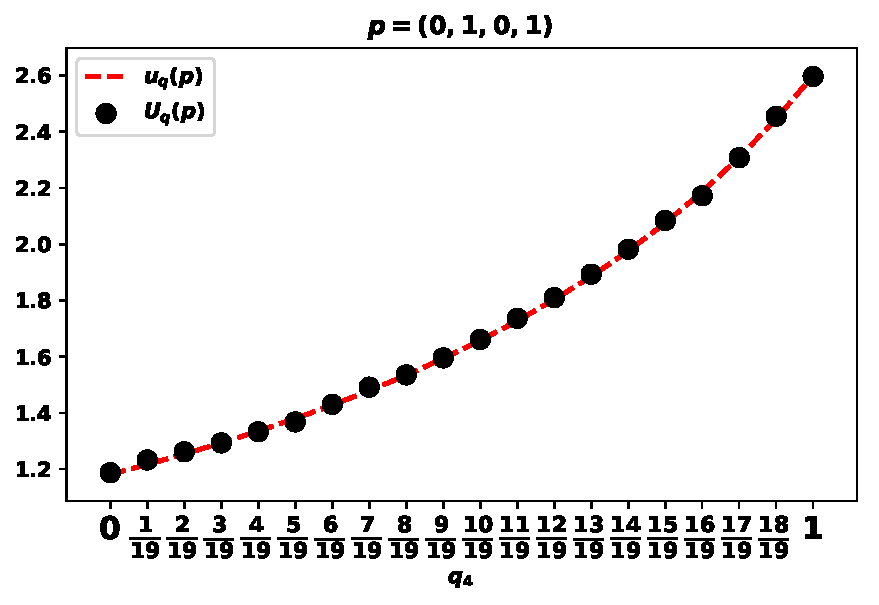
\includegraphics[width=\linewidth]{src/chapters/05/paper/Memory-size-in-the-prisoners-dilemma/img/validation_against_player_one.pdf}
        \end{subfigure}
        \begin{subfigure}{0.45\textwidth}
            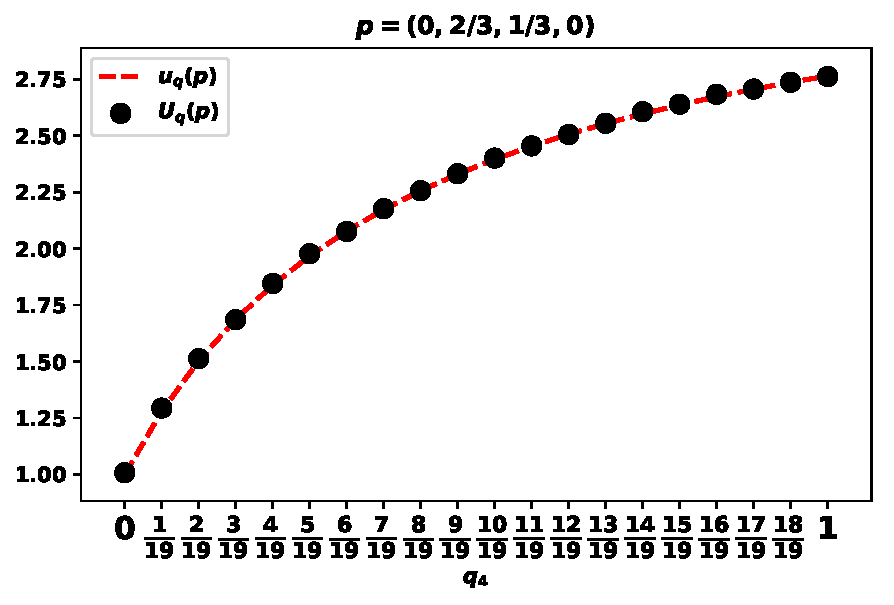
\includegraphics[width=\linewidth]{src/chapters/05/paper/Memory-size-in-the-prisoners-dilemma/img/validation_against_player_two.pdf}
        \end{subfigure}
    \end{center}
    \caption{Simulated and empirical utilities for \(p = (0, 1, 0, 1)\)
    and \(p = (0, \frac{2}{3}, \frac{1}{3}, 0)\) against \((\frac{1}{3}, \frac{1}{3}, \frac{1}{3}, q_4)\) for
    \(q_4 \in \{0,  \frac{1}{19}, \frac{2}{19}, \dots, \frac{18}{19}, 1\}\).
    \(u_q(p)\) is the theoretic value given in Theorem~\ref{theorem:quadratic_form_u},
    and \(U_q(p)\) is simulated numerically.}
    \label{fig:analytical_simulated}
\end{figure}

Theorem~\ref{theorem:quadratic_form_u} can be extended to consider multiple
opponents. The IPD is commonly studied in tournaments and/or Moran Processes
where a strategy interacts with a number of opponents. The payoff of a player in
such interactions is given by the average payoff the player received against
each opponent. More specifically the expected utility of a memory-one strategy
against a \(N\) number of opponents is given by
Theorem~\ref{theorem:tournament_utility}.

\begin{theorem}\label{theorem:tournament_utility}
    The expected utility of a memory-one strategy \(p\in\mathbb{R}_{[0,1]}^4\)
    against a group of opponents \(\{q^{(1)}, q^{(2)}, \dots, q^{(N)}\}\), denoted
    as \(\frac{1}{N} \sum\limits_{i=1} ^ {N} {u_q}^{(i)} (p)\), is given by:

    \begin{equation}\label{eq:tournament_utility}
        \frac{1}{N} \sum\limits_{i=1} ^ {N} {u_q}^{(i)} (p) = \frac{1}{N}
        \frac{\sum\limits_{i=1} ^ {N} (\frac{1}{2} pQ^{(i)} p^T + c^{(i)} p + a^ {(i)})
        \prod\limits_{\tiny\begin{array}{l} j=1 \\ j \neq i \end{array}} ^
        N (\frac{1}{2} p\bar{Q}^{(j)} p^T + \bar{c}^{(j)} p + \bar{a}^ {(j)})}
        {\prod\limits_{i=1} ^ N (\frac{1}{2} p\bar{Q}^{(i)} p^T + \bar{c}^{(i)} p + \bar{a}^ {(i)})}.
    \end{equation}
\end{theorem}

Similar to the previous result, the formulation of
Theorem~\ref{theorem:tournament_utility} is validated using numerical
simulations where the 10 memory-one strategies described in~\cite{Stewart2012}
have been used as the opponents. Figure~\ref{fig:stewart_plotkin_results} shows
that the simulated behaviour has been captured successfully.

\begin{figure}[!htbp]
    \begin{center}
    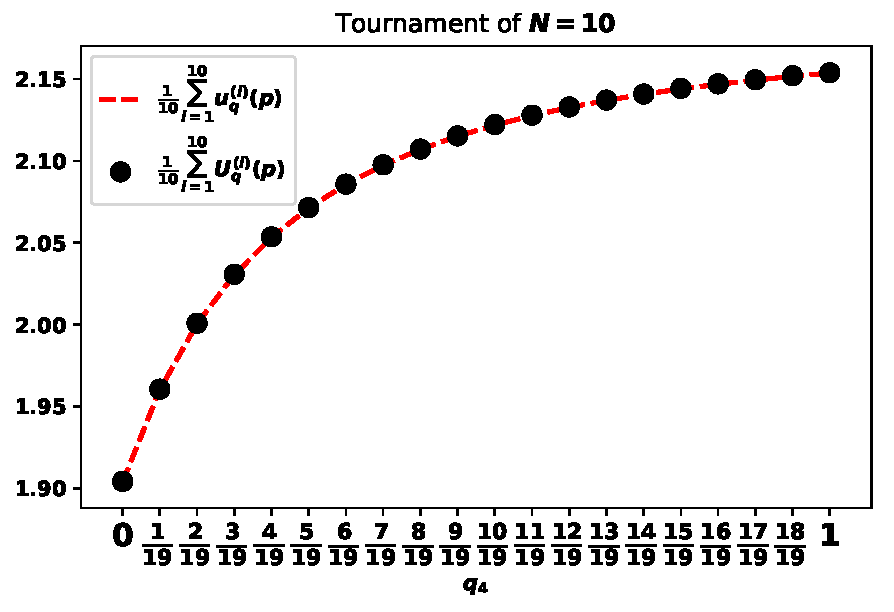
\includegraphics[width=.5\linewidth]{src/chapters/05/paper/Memory-size-in-the-prisoners-dilemma/img/Stewart_tournament_results.pdf}
    \caption{The utilities of memory-one strategies \((\frac{1}{3}, \frac{1}{3}, \frac{1}{3}, p_4)\) for
    \(p_4 \in \{0,  \frac{1}{19}, \frac{2}{19}, \dots, \frac{18}{19}, 1\}\)
    against the 10 memory-one strategies described in~\cite{Stewart2012}.
    \(\frac{1}{10} \sum^{10}_{i=1} u_q^{(i)}(p)\) is the theoretic value given in
    Theorem~\ref{theorem:quadratic_form_u},
    and \(\frac{1}{10} \sum^{10}_{i=1} U_q^{(i)}(p)\) is simulated numerically.}
    \label{fig:stewart_plotkin_results}
    \end{center}
\end{figure}

The list of strategies from~\cite{Stewart2012} was also used to check whether
the utility against a group of strategies could be captured by the utility
against the mean opponent. Thus whether condition (\ref{eq:condition}) holds.
However condition~(\ref{eq:condition}) fails, as shown in
Figure~\ref{fig:hypothesis}.

\begin{equation}\label{eq:condition}
    \frac{1}{N} \sum_{i=1} ^ {N} {u_q}^{(i)} (p) = u_{\frac {1}{N} \sum\limits_{i=1} ^ N q^{(i)}}(p),
\end{equation}

\begin{figure}[!htbp]
    \begin{center}
    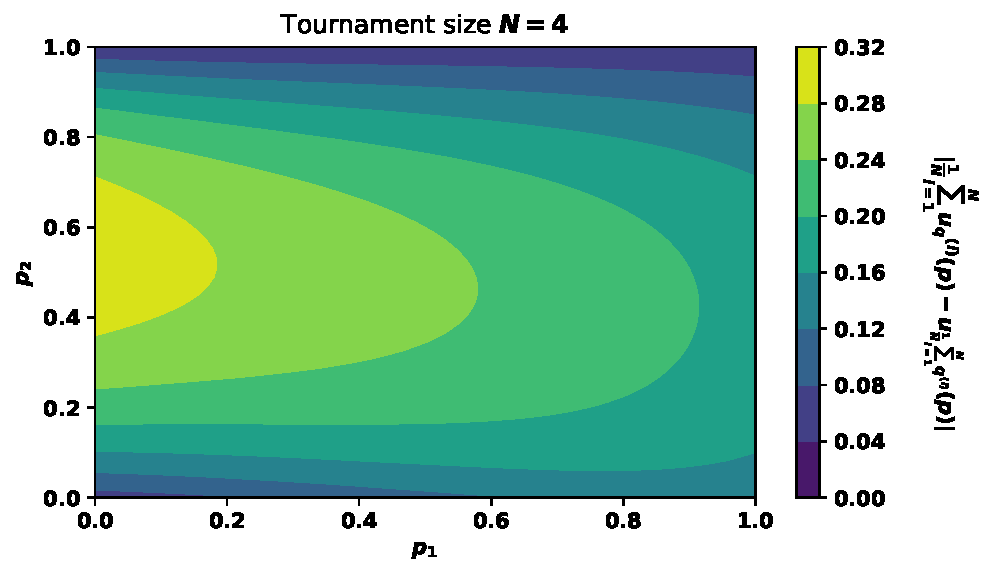
\includegraphics[width=.6\linewidth]{src/chapters/05/paper/Memory-size-in-the-prisoners-dilemma/img/mean_vs_average_heatmap.pdf}
    \end{center}
    \caption{The difference between the average utility against the opponents
    from~\cite{Stewart2012} and the utility against the average player of the
    strategies in~\cite{Stewart2012} of a player \(p=(p_1, p_2, p_1, p_2)\). A
    positive difference indicates that condition (\ref{eq:condition}) does not
    hold.}
    \label{fig:hypothesis}
\end{figure}

Theorem~\ref{theorem:tournament_utility} which allows for the utility of a
memory-one strategy against any number of opponents to be estimated without
simulating the interactions is the main result used in this Chapter. In
section~\ref{section:best_response_mem_one} it is used to define best response
memory-one strategies, in section~\ref{section:reactive_strategies} to define best response
reactive strategies and in section~\ref{section:stability_of_defection}
to explore the conditions under which defection dominates cooperation.

\section{Best responses to memory-one players}\label{section:best_response_mem_one}

This section focuses on \textit{memory-one
best response} strategies. A best response is a strategy which
corresponds to the most favourable outcome (Chapter~\ref{chapter:introduction}), thus a memory-one
best response to a set of opponents \(q^{(1)}, q^{(2)}, \dots, q^{(N)}\) corresponds to a strategy \(p^*\) for which
Equation (\ref{eq:tournament_utility}) is maximised. This is considered as a multi
dimensional optimisation problem given by:

\begin{equation}\label{eq:mo_tournament_optimisation}
    \begin{aligned}
    \max_p: & \ \sum_{i=1} ^ {N} {u_q}^{(i)} (p)
    \\
    \text{such that}: & \ p \in \R_{[0, 1]}
    \end{aligned}
\end{equation}

Optimising this particular ratio of quadratic forms is not trivial. It can be
verified empirically for the case of a single opponent that there exists at
least one point for which the definition of concavity does not hold, see Appendix~\ref{appendix:non_concave}.
The non concavity of \(u(p)\) indicates multiple local
optimal points. This is also intuitive. The best response against a cooperator,
\(q=(1, 1, 1, 1)\), is a defector \(p^*=(0, 0, 0, 0)\). The strategies
\(p=(\frac{1}{2}, 0, 0, 0)\) and \(p=(\frac{1}{2}, 0, 0, \frac{1}{2})\) are also
best responses. The approach taken here is to introduce a compact way of
constructing the discrete candidate set of all local optimal points, and evaluating
the objective function Equation~(\ref{eq:tournament_utility}). This gives the best
response memory-one strategy. The approach is given in
Theorem~\ref{theorem:memone_group_best_response}.

\begin{theorem}\label{theorem:memone_group_best_response}

    The optimal behaviour of a memory-one strategy
    \(p^* \in \R_{[0, 1]} ^ 4\)
    against a set of \(N\) opponents \(\{q^{(1)}, q^{(2)}, \dots, q^{(N)} \}\)
    for \(q^{(i)} \in \R_{[0, 1]} ^ 4\) is given by:

    \[p^* = \textnormal{argmax}\sum\limits_{i=1} ^ N  u_q(p), \ p \in S_q.\]

    The set \(S_q\) is defined as all the possible combinations of:

    \begin{equation}\label{eq:s_q_set}
        \resizebox{.9\linewidth}{!}{ $
        S_q =
        \left\{p \in \mathbb{R} ^ 4 \left|
            \begin{aligned}
                \bullet\quad p_j \in \{0, 1\} & \quad \text{and} \quad \frac{d}{dp_k} 
                \sum\limits_{i=1} ^ N  u_q^{(i)}(p) = 0
                \quad \text{for all} \quad j \in J \quad \&  \quad k \in K  \quad \text{for all} \quad J, K \\
                & \quad \text{where} \quad J \cap K = \O \quad
                \text{and} \quad J \cup K = \{1, 2, 3, 4\}.\\
                \bullet\quad  p \in \{0, 1\} ^ 4
            \end{aligned}\right.
        \right\}.
        $}
    \end{equation}
\end{theorem}

\begin{proof}
The optimal behaviour of a memory-one strategy player
\(p^* \in \R_{[0, 1]} ^ 4\)
against a set of \(N\) opponents \(\{q^{(1)}, q^{(2)}, \dots, q^{(N)} \}\)
for \(q^{(i)} \in \R_{[0, 1]} ^ 4\) is established by:

\[p^* = \textnormal{argmax}\left(\sum\limits_{i=1} ^ N  u_q(p)\right), \ p \in S_q,\]

where \(S_q\) is given by Equation~(\ref{eq:s_q_set}).

The optimisation problem of (\ref{eq:mo_tournament_optimisation}) can be
written as:

\begin{equation}\label{eq:mo_tournament_optimisation_standard}
    \begin{aligned}
    \max_p: & \ \sum_{i=1} ^ {N} {u_q}^{(i)} (p)
    \\
    \text{such that}: p_i & \leq 1 \text{ for } \in \{1, 2, 3, 4\} \\
    - p_i & \leq 0 \text{ for } \in \{1, 2, 3, 4\} \\
    \end{aligned}
\end{equation}

The optimisation problem has two inequality constraints and regarding the optimality
this means that:

\begin{itemize}
    \item either the optimum is away from the boundary of the optimization domain, and so the constraints plays no role;
    \item or the optimum is on the constraint boundary.
\end{itemize}

Thus, the following three cases must be considered:

\textbf{Case 1:} The solution is on the boundary and any of the possible
combinations for $p_i \in \{0, 1\}$ for $i \in \{1, 2, 3, 4\}$ are candidate
optimal solutions.

\textbf{Case 2:} The optimum is away from the boundary of the optimization domain
and the interior solution $p^*$ necessarily satisfies the condition
\(\frac{d}{dp} \sum\limits_{i=1} ^ N  u_q(p^*) = 0\).

\textbf{Case 3:} The optimum is away from the boundary of the optimization domain
but some constraints are equalities. The candidate solutions in this case
are any combinations of $p_j \in \{0, 1\} \quad \text{and} \quad \frac{d}{dp_k} 
\sum\limits_{i=1} ^ N  u_q^{(i)}(p) = 0$ 
for all $ j \in J \text{ \& } k \in K \text{ for all } J, K
\text{ where } J \cap K = \O \text{ and } J \cup K = \{1, 2, 3, 4\}.$

Combining cases 1-3 a set of candidate solution is constructed as:

\begin{equation*}
    \resizebox{\linewidth}{!}{ $
    S_q =
    \left\{p \in \mathbb{R} ^ 4 \left|
        \begin{aligned}
            \bullet\quad p_j \in \{0, 1\} & \quad \text{and} \quad \frac{d}{dp_k} 
            \sum\limits_{i=1} ^ N  u_q^{(i)}(p) = 0
            \quad \text{for all} \quad j \in J \quad \&  \quad k \in K  \quad \text{for all} \quad J, K \\
            & \quad \text{where} \quad J \cap K = \O \quad
            \text{and} \quad J \cup K = \{1, 2, 3, 4\}.\\
            \bullet\quad  p \in \{0, 1\} ^ 4
        \end{aligned}\right.
    \right\}.
    $}
\end{equation*}

The derivative of \(\sum\limits_{i=1} ^ N  u_q^{(i)}(p)\) calculated using
the following property (see~\cite{Abadir2005} for details):

\begin{equation}\label{eq:first_derivative_property}
\frac{d x A x^T}{dx} =  2Ax.
\end{equation}

Using property~(\ref{eq:first_derivative_property}):

\begin{equation}\label{eq:quadratics_derivatives}
\frac{d}{dp} \frac{1}{2}pQp^T + cp + a = pQ + c \text{ and } \frac{d}{dp} \frac{1}{2}p\bar{Q}p^T + \bar{c}p + \bar{a} = p\bar{Q} + \bar{c}.
\end{equation}

Note that the derivative of \(cp\) is \(c\) and the constant disappears.
Combining these it can be proven that:

\begin{equation*}
\resizebox{\textwidth}{!}{$ \begin{split}
\frac{d}{dp} \sum\limits_{i=1} ^ N  u_q^{(i)}(p) & = \sum\limits_{i=1} ^ N \frac{\frac{d}{dp}(\frac{1}{2}pQ^{(i)}p^T + c^{(i)}p + a^{(i)} )(\frac{1}{2}p\bar{Q}^{(i)}p^T + \bar{c}^{(i)}p + \bar{a}^{(i)}) -
\frac{d}{dp}(\frac{1}{2}p\bar{Q}^{(i)}p^T + \bar{c}^{(i)}p + \bar{a}^{(i)})(\frac{1}{2}pQ^{(i)}p^T + c^{(i)}p + a^{(i)})}{(\frac{1}{2}p\bar{Q}^{(i)}p^T + \bar{c}^{(i)}p + \bar{a}^{(i)})^2} \\
& = \sum\limits_{i=1} ^ N \frac{(pQ^{(i)} + c^{(i)} +)(\frac{1}{2}p\bar{Q}^{(i)}p^T + \bar{c}^{(i)}p + \bar{a}^{(i)})}{(\frac{1}{2}p\bar{Q}^{(i)}p^T + \bar{c}^{(i)}p + \bar{a}^{(i)})^2} -
 \frac{(p\bar{Q}^{(i)}+ \bar{c}^{(i)})(\frac{1}{2}pQ^{(i)}p^T + c^{(i)}p + a^{(i)})}{(\frac{1}{2}p\bar{Q}^{(i)}p^T + \bar{c}^{(i)}p + \bar{a}^{(i)})^2}
\end{split}$}
\end{equation*}

For \(\frac{d}{dp} \sum\limits_{i=1} ^ N  u_q(p)\) to equal zero then:

{\scriptsize
\begin{align}\label{eq:polynomials_roots}
    \displaystyle\sum\limits_{i=1} ^ {N}
    \left(pQ^{(i)} + c^{(i)}\right) \left(\frac{1}{2} p\bar{Q}^{(i)} p^T + \bar{c}^{(i)} p + \bar{a}^ {(i)}\right)
    - \left(p\bar{Q}^{(i)} + \bar{c}^{(i)}\right) \left(\frac{1}{2} pQ^{(i)} p^T + c^{(i)} p + a^ {(i)}\right)
    & = 0, \quad {while} \\
    \displaystyle\sum\limits_{i=1} ^ {N} \frac{1}{2} p\bar{Q}^{(i)} p^T + \bar{c}^{(i)} p + \bar{a}^ {(i)} & \neq 0.
\end{align}}

The optimal solution to Equation~\ref{eq:mo_tournament_optimisation} is the point
from $S_q$ for which the utility is maximised.

\end{proof}

Note that there is no immediate way to find the zeros of \(\frac{d}{dp} \sum\limits_{i=1} ^ N  u_q(p)\);

{\small
\begin{align}\label{eq:mo_tournament_derivative}
    \frac{d}{dp} \sum\limits_{i=1} ^ {N} {u_q}^{(i)} (p) & = \nonumber \\
    & =  \displaystyle\sum\limits_{i=1} ^ {N}
    \frac{\left(pQ^{(i)} + c^{(i)}\right) \left(\frac{1}{2} p\bar{Q}^{(i)} p^T + \bar{c}^{(i)} p + \bar{a}^ {(i)}\right)
    - \left(p\bar{Q}^{(i)} + \bar{c}^{(i)}\right) \left(\frac{1}{2} pQ^{(i)} p^T + c^{(i)} p + a^ {(i)}\right)}
    {\left(\frac{1}{2} p\bar{Q}^{(i)} p^T + \bar{c}^{(i)} p + \bar{a}^ {(i)}\right)^ 2}
\end{align}
}

For \(\frac{d}{dp} \sum\limits_{i=1} ^ N  u_q(p)\) to equal zero then:

{\scriptsize
\begin{align}\label{eq:polynomials_roots}
    \displaystyle\sum\limits_{i=1} ^ {N} \left(
    \left(pQ^{(i)} + c^{(i)}\right) \left(\frac{1}{2} p\bar{Q}^{(i)} p^T + \bar{c}^{(i)} p + \bar{a}^ {(i)}\right)
    - \left(p\bar{Q}^{(i)} + \bar{c}^{(i)}\right) \left(\frac{1}{2} pQ^{(i)} p^T + c^{(i)} p + a^ {(i)}\right)\right)
    &= 0, \quad {while} \\
    \displaystyle\sum\limits_{i=1} ^ {N} \frac{1}{2} p\bar{Q}^{(i)} p^T + \bar{c}^{(i)} p + \bar{a}^ {(i)} &\neq 0.
\end{align}}

Finding best response memory-one strategies, more specifically constructing the
subset \(S_q\), can be done analytically. The points for any or all of \(p_i \in
\{0, 1\}\) for \(i \in \{1, 2, 3, 4\}\) are trivial, and finding the
roots of the partial derivatives which are a set of polynomials of Equations
(\ref{eq:polynomials_roots}) is feasible using resultant
theory~\cite{Jonsson2005}; however, for large systems building the resultant
quickly becomes intractable.

Nevertheless, there are constrained versions of problem
(\ref{eq:mo_tournament_optimisation}) for which calculating
the resultant is efficient and a best response strategy can be identified
explicitly. A constrained version is that of reactive strategies.
Section~\ref{section:reactive_strategies} presents best response
reactive strategies, and demonstrates the usage of resultant theory in
identifying best responses.

\section{Reactive Strategies \& Resultant Theory}\label{section:reactive_strategies}

Reactive strategies are a subset of memory-one strategies discussed
in Chapter~\ref{chapter:literature_review}. Well known reactive strategies
include Tit For Tat and Generous Tit for Tat. As a reminder, reactive strategies
only take into account the opponent's previous moves, and thus can be described
as \(p = (p_1, p_2) \in R^2\).

\textit{Best response reactive} strategies are incorporated in the formulation of
this Chapter by adding two extra constraints to the
optimisation problem of (\ref{eq:mo_tournament_optimisation}),

\begin{equation}\label{eq:reactive_tournament_optimisation}
\begin{aligned}
\max_p: & \ \sum_{i=1} ^ N u_q(p)
\\
\text{such that}: & \ p_1 = p_3 \\
                  & \ p_2 = p_4\\
                  & \ p_1, p_2 \in \R_{[0, 1]}.
\end{aligned}
\end{equation}

and a best response reactive strategy to a set of opponents \(N\) opponents
\(\{q^{(1)}, q^{(2)}, \dots, q^{(N)} \}\) is given by
Lemma~\ref{lemma:reactive_best_response}.

\begin{lemma}\label{lemma:reactive_best_response}
    The optimal behaviour of a reactive strategy
    \(p^* \in \R_{[0, 1]} ^ 2\)
    against a set of \(N\) opponents \(\{q^{(1)}, q^{(2)}, \dots, q^{(N)} \}\)
    for \(q^{(i)} \in \R_{[0, 1]} ^ 2\) is given by:

    \[p^* = \textnormal{argmax}\sum\limits_{i=1} ^ N  u_q(p), \ p \in S_q.\]

    The set \(S_q\) is defined as all the possible combinations of:
    
    \begin{equation}\label{eq:s_q_reactive_set}
        \resizebox{.9\linewidth}{!}{ $
        S_q =
        \left\{p \in \mathbb{R} ^ 2 \left|
            \begin{aligned}
                \bullet\quad p_j \in \{0, 1\} & \quad \text{and} \quad \frac{d}{dp_k} 
                \sum\limits_{i=1} ^ N  u_q^{(i)}(p) = 0
                \quad \text{for all} \quad j \in J \quad \&  \quad k \in K  \quad \text{for all} \quad J, K \\
                & \quad \text{where} \quad J \cap K = \O \quad
                \text{and} \quad J \cup K = \{1, 2\}.\\
                \bullet\quad  p \in \{0, 1\} ^ 2
            \end{aligned}\right.
        \right\}.
        $}
    \end{equation}
\end{lemma}

Note that \(\frac{d}{dp} \sum\limits_{i=1} ^ N  u_q^{(i)}(p) = 0\) corresponds
to a system of 2 polynomials of 2 variables, corresponding to the partial
derivatives over \(p_1\) and \(p_2\). Solving systems of 2 polynomial of 2
variables can be done analytically. The approach taken here to extract the roots
from the partial derivatives is that of the resultant.

\subsection{Resultant Theory}

The \textit{resultant} of two polynomials is a polynomial expression of
their coefficients which is equal to zero if and only if the polynomials have a
common root. 

More specifically given a polynomial,

\[ f(x) = a_n x^n + a_{(n-1)} x ^{(n-1)} + \dots +a_1 x + a_0 \]

of degree \(n\) with roots \(\alpha_i, i=1, \dots, n\) and a polynomial

\[ g(x) = b_m x ^m + b_{(m-1)} x^{(m-1)} + \dots + b_1 x + b_0 \]

of degree m with roots \(\beta_j, j=1, \dots , m,\) the resultant denoted as \(R(f, g)\)
and also called the eliminant~\cite{Salmon1924}, is defined by

\begin{equation}\label{eq:resultant_definition}
R(f, g) = a_n^m b_m^n \prod_{(i=1)}^n \prod_{(j=1)}^m ( \alpha_i - \beta_j).
\end{equation}

Interestingly, the resultant of can also be expressed as the determinant of
matrices such as the Sylvester's, the Bezout's and the Macaulay's. For systems
of 2 polynomials the resultant is commonly expressed as the determinant of the
Sylvester's matrix~\cite{Akritas2014}. The Sylvester matrix associated with
\(f\) and \(g\) is the \((n + m) \times (n + m)\) matrix constructed as
described in Algorithm~\ref{algorithm:sylvester}.

\begin{algorithm}[H]
    \If{\(n > 0\)}{
        the \(1^{\text{st}}\) row is $\begin{pmatrix} a_{m} & a_{{m-1}} & \cdots & a_{1} & a_{0} & 0 & \cdots & 0\end{pmatrix}$ \;
        \For{$i\gets1$ \KwTo $n-1$}{the \(i^{\text{th}}\) is the previous row shifted one column to the right; the other entries of the row are 0} \;}
    \If{\(m > 0\)}{
        the \((n + 1)^{\text{th}}\) is: $\begin{pmatrix} b_{m} & b_{{m-1}} & \cdots & b_{1} & b_{0} & 0 & \cdots & 0\end{pmatrix}$ \;
        \For{$i\gets n+1$ \KwTo $(m + n)-1$}{the \(i^{\text{th}}\) is the previous row shifted one column to the right; the other entries of the row are 0}}
\caption{Construction of Sylvester matrix~\cite{Akritas2014}}\label{algorithm:sylvester}
\end{algorithm}

As an example consider the case of \(m = 4\) and \(n = 3\). The Sylvester matrix
denoted as \(S_{f,g}\) is given by,

\begin{equation}
S_{f,g} = \begin{pmatrix} a_{4} & a_{3} & a_{2} & a_{1} & a_{0} & 0     & 0    \\
                          0     & a_{4} & a_{3} & a_{2} & a_{1} & a_{0} & 0    \\
                          0     & 0     & a_{4} & a_{3} & a_{2} & a_{1} & a_{0} \\
                          b_{3} & b_{2} & b_{1} & b_{0} &     0 & 0     & 0     \\
                          0     & b_{3} & b_{2} & b_{1} & b_{0} & 0     & 0     \\
                          0     & 0     & b_{3} & b_{2} & b_{1} & b_{0} & 0     \\
                          0     & 0     & 0     & b_{3} & b_{2} & b_{1} & b_{0}
                        \end{pmatrix}
\end{equation}

and,

\[|S_{f, g}| = R(f, g).\]

The resultant can assure that a system has root, nevertheless, it can also be
used to extract those roots. In a system of 2 polynomial equations in 2
variables, the resultant can be defined over one variable whereas the second one
is kept as a coefficient. It is used in this Chapter to analytically solve for
the roots of the utility, and thus explicitly identify the best response
reactive strategy against a given set of memory-one opponents.

The open source package~\cite{sympy} is used to calculate the Sylvester matrix
and subsequently it's determinant. An example is demonstrated in
Figure~\ref{figure:code_for_sylvester}.

\begin{figure}[!htbp]
    \begin{usagepy}
>>> p_1 = sym.symbols('p_1')
>>> p_2 = sym.symbols('p_2')

>>> f = p_1 ** 2 + p_1 * p_2 + 2 * p_1 + p_2 - 1
>>> g = p_1 ** 2 + 3 * p_1 - p_2 ** 2 + 2 * p_2 - 1
>>> matrix = subresultants_qq_zz.sylvester(f, g, p_2)
>>> matrix
Matrix([
[p_1 + 1, p_1**2 + 2*p_1 - 1,                  0],
[      0,            p_1 + 1, p_1**2 + 2*p_1 - 1],
[     -1,                  2, p_1**2 + 3*p_1 - 1]])
>>> matrix.det().factor()
-p_1*(p_1 - 1)*(p_1 + 3)
\end{usagepy}
    \caption{Example code for calculating the Sylvester matrix associated with
    \(f = p_1^2 + p_1 p_2 + 2 p_1 + p_2 - 1\) and \(g = p_1^2 + 3 p_1 - p_2^2 +
    2p_2 - 1\) using~\cite{sympy}. The matrix is calculated for \(p_2\) whilst
    \(p_1\) is handled as a coefficient, and thus the determinant is expressed
    in \(p_1\). In order for the system to have a common root, \(p_1\) must be
    \(\in \{-3, 0, 1\}\). By substituting these values of \(p_1\), each at a
    time, in \(f\) and \(g\) gives the roots for
    \(p_2\).}\label{figure:code_for_sylvester}
\end{figure}

The approach demonstrated in Figure~\ref{figure:code_for_sylvester} is used to
find the roots of the partial derivatives of \(\frac{d}{dp} \sum\limits_{i=1} ^
N  u_q^{(i)}(p)\) and the candidate set of solutions \(S_q\) is constructed
as defined in Equation~(\ref{eq:s_q_reactive_set}).

A bespoke package has been developed to carry out the calculations for this
Chapter. The package is called \mintinline{python}{opt_mo} and an example of
how \(S_q\) is calculated against a given opponent \(q =
(0.513, 0.773, 0.870, 0.008)\) is given by
Figure~\ref{fig:reactive_example_get_candidate_set}.

\begin{figure}[!htbp]
\begin{usagepy}
>>> import opt_mo
>>> axl.seed(14)
>>> opponent = [np.random.random(4)]
>>> opponent
[array([0.51394334, 0.77316505, 0.87042769, 0.00804695])]

>>> candidate_set = opt_mo.reactive_best_response.get_candidate_reactive_best_responses(opponents)
>>> candidate_set
{0, 0.2775453690890986, 0.6964731896521483, (0.913428410721382+0j), 1}
\end{usagepy}
\caption{Code example of calculating \(S_q\) for a given opponent. The function
\mintinline{python}{reactive_best_response.get_candidate_reactive_best_responses}
retrieves the set \(S_q\) for a reactive strategy against a list of opponents.
The set includes \(0\), \(1\) and to roots of the partial derivatives
\(0.2775453690890986, 0.6964731896521483\). An imaginary solution has also been
calculated, however, it is ignore in the next step which calculates the best
response.}\label{fig:reactive_example_get_candidate_set}
\end{figure}

Once \(S_q\) is calculated then defining the best response is trivial.
Figure~\ref{fig:reactive_example_best_response} demonstrates how this is done
using \mintinline{python}{opt_mo}, and the result is validated by
Figure~\ref{fig:reactive_example_utility}.

\begin{figure}[!htbp]
    \begin{usagepy}
>>> opt_p1, opt_p2, score = opt_mo.reactive_best_response.get_argmax(opponents, candidate_set)
>>> opt_p1, opt_p2 (0,0.6964731896521483)
\end{usagepy}
\caption{Code example of estimating the best response
reactive strategy from a given \(S_q\) set and a given list of
opponents.}\label{fig:reactive_example_best_response}
\end{figure}

\begin{figure}[!htbp]
    \centering
    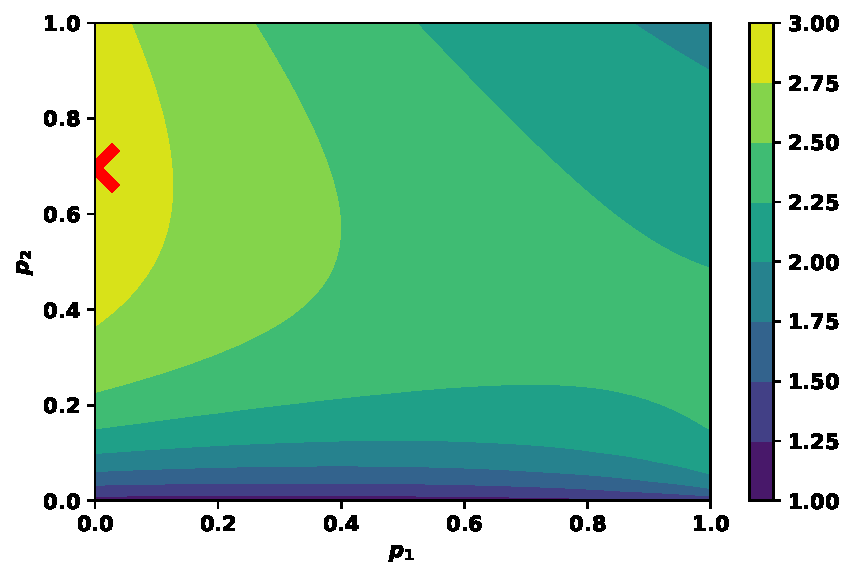
\includegraphics[width=.6\linewidth]{src/chapters/05/reactive_best_response.pdf}
    \caption{The utility of a \(p=(p_1, p_2)\) reactive player against \(q =
    (0.513, 0.773, 0.870, 0.008)\) for changing values of \(p_1\) and \(p_2\).
    The point marked with X is the point identified as the best response.}
    \label{fig:reactive_example_utility}
\end{figure}

Sylvester's formulation can only handle systems of 2 polynomials, however, the
resultant can still be calculated for \(n\) homogeneous polynomials in \(n\)
variables and it's called \textit{multivariate resultant}. A number of
multivariate resultants can be found in the literature such as
Dixon's~\cite{ResultantKapur} resultant and the Macaulay's~\cite{Macaulay1902}
resultant.

Project~\cite{sympy} which was used to construct Sylvester's resultant is called
SymPy and it is the Pythonic package for symbolic mathematics. However, the
project did not be include the feature to calculate multivariate resultant. As
part of this Chapter the source code for constructing both the Dixon's and
Macaulay's resultants was developed and was integrated into
project~\cite{sympy}. Figure~\ref{fig:dixon_example} demonstrates an example of
using~\cite{sympy} to calculate Dixon's resultant.

\begin{figure}
\begin{usagepy}
>>> from sympy.polys.multivariate_resultants import DixonResultant
>>> f = x + y
>>> g = x ** 2 + y ** 3
>>> h = x ** 2 + y
>>> matrix = DixonResultant(variables=[x, y], polynomials=[p, q, h])
>>> matrix.det()
0 
\end{usagepy}
\caption{Code example of using~\cite{sympy} to calculate Dixon's resultant.
\(f, g\) and \(h\) have a common root (\(x=1, y=-1\)). The determinant
of Dixon's matrix falls to zero which confirms that the system has a common root.}\label{fig:dixon_example}
\end{figure}

Multivariate resultants theoretically can be used to explicitly identify best
response memory one strategies, but solving a system of 4 polynomials. However,
as previously stated for large systems building the resultant quickly becomes
intractable. As a result in section~\ref{section:numerical_experiments}
a numerical approach was considered instead.

\section{Numerical experiments} \label{section:numerical_experiments}

The results of this section rely on estimating best response memory-one strategies, but as stated in
Section~\ref{section:best_response_mem_one}, estimating best responses
analytically can quickly become an intractable problem. As a result, best
responses will be estimated heuristically using Bayesian
optimisation~\cite{Mokus1978}. 

\subsection{Bayesian optimisation}

Bayesian optimisation is a global optimisation
algorithm that has proven to outperform many other popular
algorithms~\cite{Jones2001}. The algorithm builds a bayesian understanding of
the objective function which is well suited to the potential multiple local optimas in
the described search space of this work. Differential evolution~\cite{Storn1997}
was also considered, however, it was not selected due to Bayesian optimisation being
computationally more efficient.

As an example of the algorithm's usage consider the optimisation problem
of (\ref{eq:mo_tournament_optimisation}). Figure~\ref{bayesian_example}
illustrates the change of the utility function over iterations of the algorithm.
The algorithm is set to run for 60 iterations. After 60 iterations if the
utility has changed in the last 10\% iterations then algorithm runs for a
further 20 iterations. This is repeated until there is no change to the utility
in the last 10\% of iterations.


\begin{figure}[!htbp]
    \begin{center}
    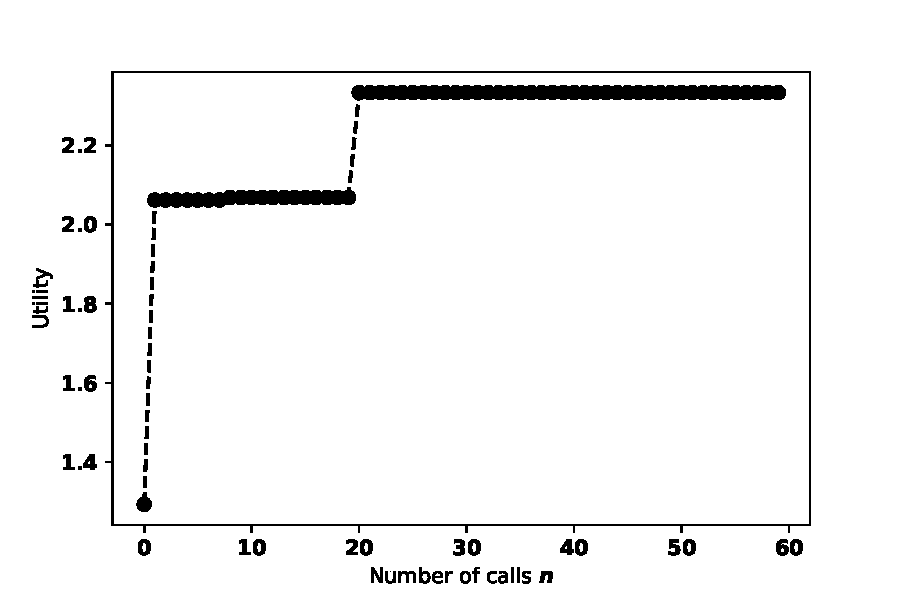
\includegraphics[width=.5\linewidth]{src/chapters/05/paper/Memory-size-in-the-prisoners-dilemma/img/bayesian_example.pdf}
    \end{center}
    \caption{Utility over time of calls using Bayesian optimisation. The
    opponents are \(q^{(1)} = (\frac{1}{3}, \frac{1}{3}, \frac{1}{3},
    \frac{1}{3})\) and \(q^{(2)} = (\frac{1}{3}, \frac{1}{3},
    \frac{1}{3}, \frac{1}{3})\). The best response obtained is \(p^* = (0, \frac{11}{50}, 0, 0)\)}
    \label{bayesian_example}
\end{figure}

\subsection{SSE Method}

In order to investigate whether best responses
behave in an extortionate matter the SSE method~\cite{Knight2019} is used. More
specifically,
in~\cite{Knight2019} a point \(x^*\), in the space of memory-one strategies, is
defined as the nearest extortionate strategy to a given strategy \(p\). \(x^*\) is
given by,

\begin{equation}\label{eqn:x_star_formula}
    x^* = {\left(C^{T}C\right)}^{-1}C^{T}\bar{p}
\end{equation}

where \(\bar{p}=(p_1 - 1, p_2 - 1, p_3, p_4)\) and

\begin{equation}\label{eq:definition_of_C}
    C =
    \begin{bmatrix}
        R - P & R- P \\
        S - P & T- P \\
        T - P & S- P \\
        0     & 0 \\
    \end{bmatrix}.
\end{equation}

The squared norm of the remaining error is referred to as sum of squared errors
of prediction (SSE):

\begin{equation}\label{eqn:x_SSError_formula}
    \text{SSE} = {\bar{p}} ^ T \bar{p} -
           \bar{p} C \left(C ^ T C \right) ^ {-1} C ^ T \bar{p}
         = {\bar{p}} ^ T \bar{p} - \bar{p} C x ^ *
\end{equation}

Thus, SSE is defined as how far a strategy is from behaving as a ZD and thus a
high SSE implies a non extortionate behaviour. The SSE method has been applied
to the data set. A statistics summary of the SSE distribution for the best
response in tournaments and evolutionary dynamics is given in
Table~\ref{table:sserror_stats}.

The rest of the section is structured as follows. In
section~\ref{subsection:best_response_n_2}, Bayesian optimisation is used to
generate a data set containing memory-one best responses against a number of
random opponents. The extortionate behaviour of these best responses is then
evaluated using a method introduced in~\cite{Knight2019}. In section
\ref{subsection:best_respnse_evolutionary_setting}, a similar data set and
approach are discussed but this time the best responses are memory-one best
responses in an evolutionary setting where they also incorporate self
interactions. This has immediate applications to Moran processes.
Finally, section~\ref{subsection:longer_memory_best_response}
compares the performances of memory-one and longer-memory best responses against
a number of opponents.

\subsection{Best response memory-one strategies for \(N=2\)}\label{subsection:best_response_n_2}

As briefly discussed in section~\ref{section:introduction}, ZDs
have been praised for their robustness against a single opponent.
ZDs are evidence that extortion works in pairwise interactions.
Their behaviour ensures that the strategies will
never lose a game. However, this thesis
argues that in multi opponent interactions, where the payoffs matter, strategies
trying to exploit their opponents will suffer.

Compared to ZDs, best response memory-one strategies which
have a theory of mind of their opponents, utilise their behaviour in order to
gain the most from their interactions. The question that arises then is whether
best response strategies are optimal because they behave in an extortionate
way. To estimate a strategy's extortionate
behaviour the SSE method as described in~\cite{Knight2019} is used. SSE is
defined as how far a strategy is from behaving extortionate, thus a high
SSE implies a non extortionate behaviour.

A data set of best response memory-one strategies with \(N=2\) opponents has been
generated which is available at~\cite{glynatsi2019}. The data set contains a total of 1000 trials
corresponding to 1000 different instances of a best response strategy. For each
trial a set of 2 opponents is randomly generated and the memory-one best response
against them is found. The probabilities \(q_i\) of the opponents are
randomly generated and Figures~\ref{fig:first_opponents_probabilities} and
\ref{fig:second_opponents_probabilities}, show that they are uniformly
distributed over the trials. Thus, the full space of possible opponents has been
covered.

\begin{figure}[!htbp]
    \begin{subfigure}{0.47\textwidth}
        \centering
        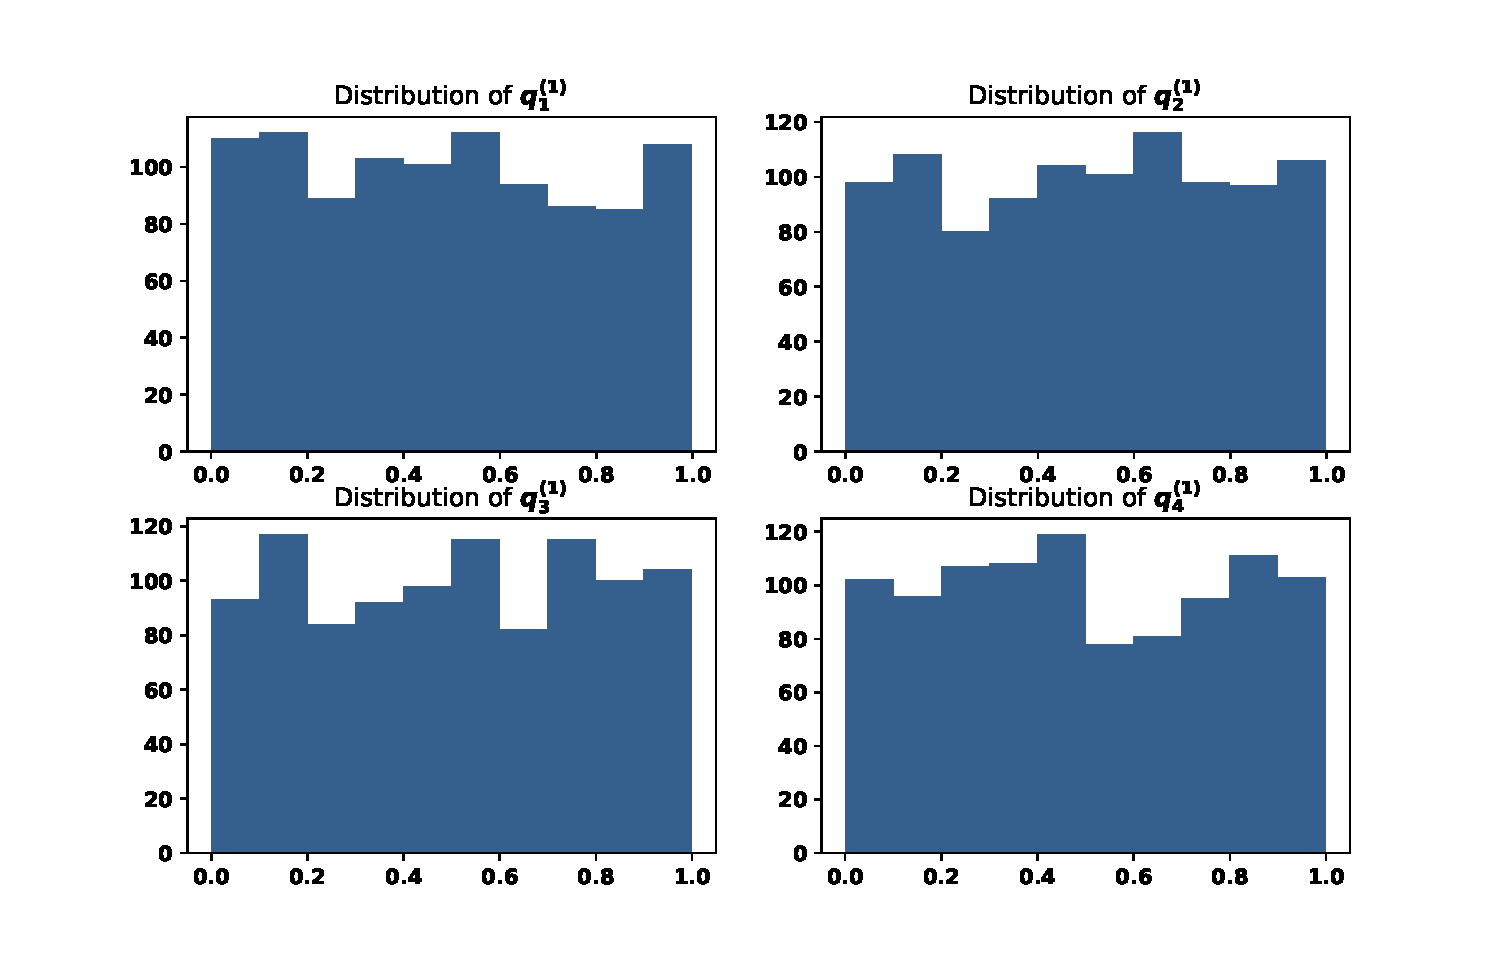
\includegraphics[width=\linewidth]{src/chapters/05/paper/Memory-size-in-the-prisoners-dilemma/img/first_opponent_probabilities.pdf}
        \subcaption{Distributions of first opponents' probabilities.}
        \label{fig:first_opponents_probabilities}
    \end{subfigure}\hfill
    \begin{subfigure}{0.47\textwidth}
        \centering
        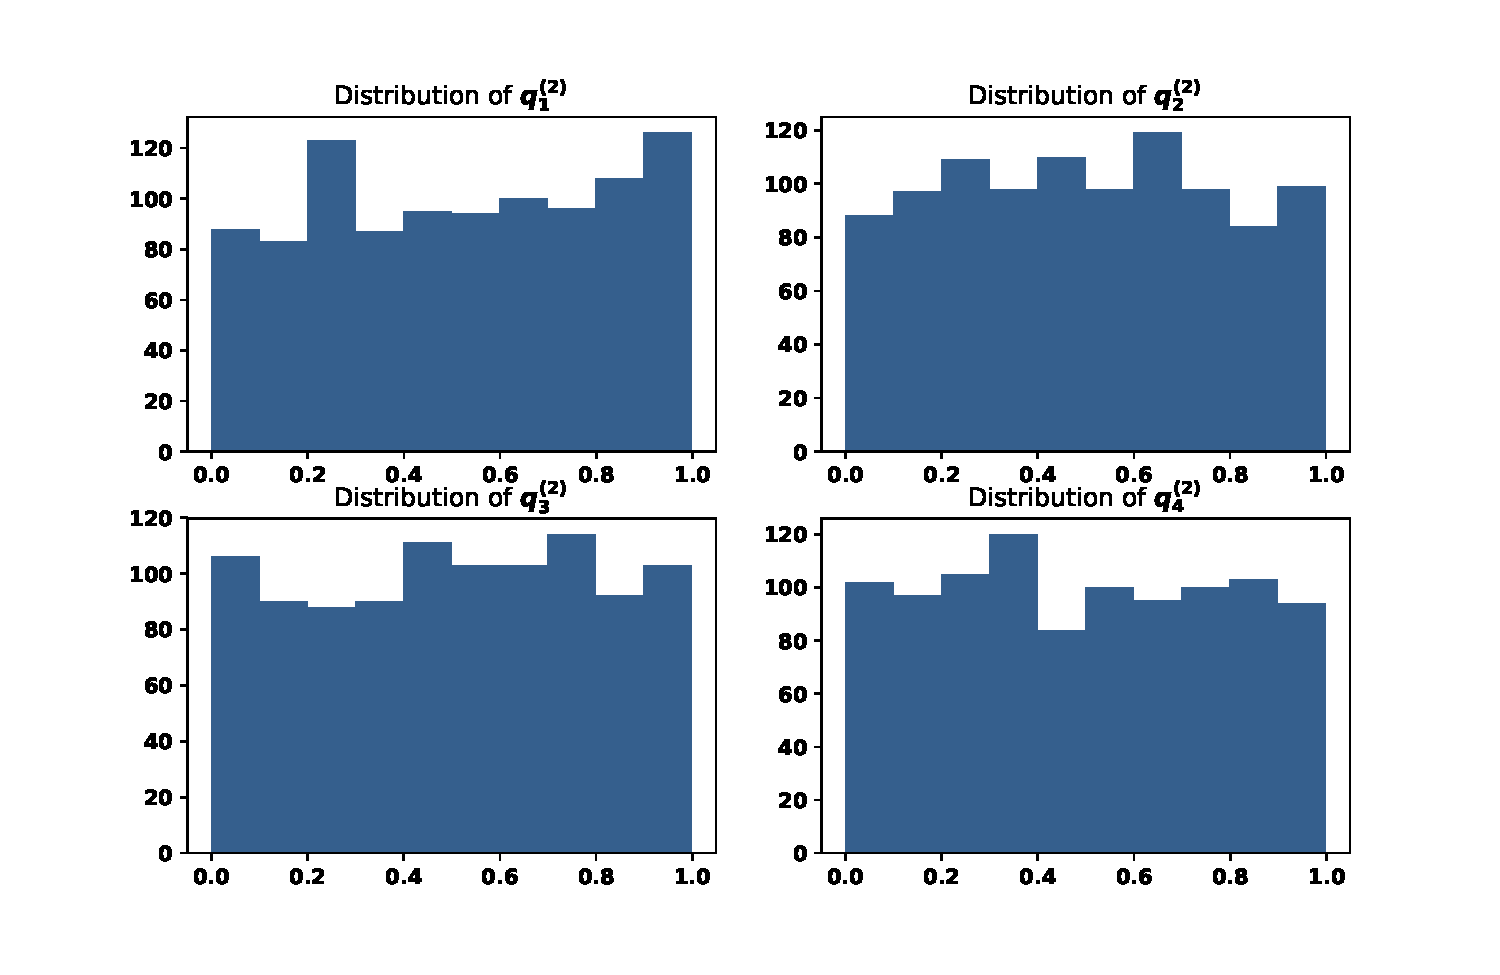
\includegraphics[width=\linewidth]{src/chapters/05/paper/Memory-size-in-the-prisoners-dilemma/img/second_opponent_probabilities.pdf}
        \subcaption{Distributions of second opponents' probabilities.}
        \label{fig:second_opponents_probabilities}
    \end{subfigure}
\end{figure}

The SSE method has been applied to the data set. The distribution of SSE for the best response is given in
Figure~\ref{fig:sserror_mem_one} and a statistics summary in
Table~\ref{table:sserror_stats}. The distribution of SSE is skewed to the left,
indicating that the best response does exhibit extortionate behaviour, however,
the best response is not uniformly extortionate. A positive measure of skewness
and kurtosis indicates a heavy tail to the right. Therefore, in several cases the
strategy is not trying to extort its the opponents.

So although the best response strategy can exhibit extortionate behaviour, its
performance is maximised by behaving in a more adaptable way than zero-determinant
strategies. This is confirms similar results such as~\cite{Knight2019}.
This analysis will now be extended to an evolutionary setting.

\begin{figure}[!htbp]
    \begin{minipage}{0.65\textwidth}
            \begin{center}
                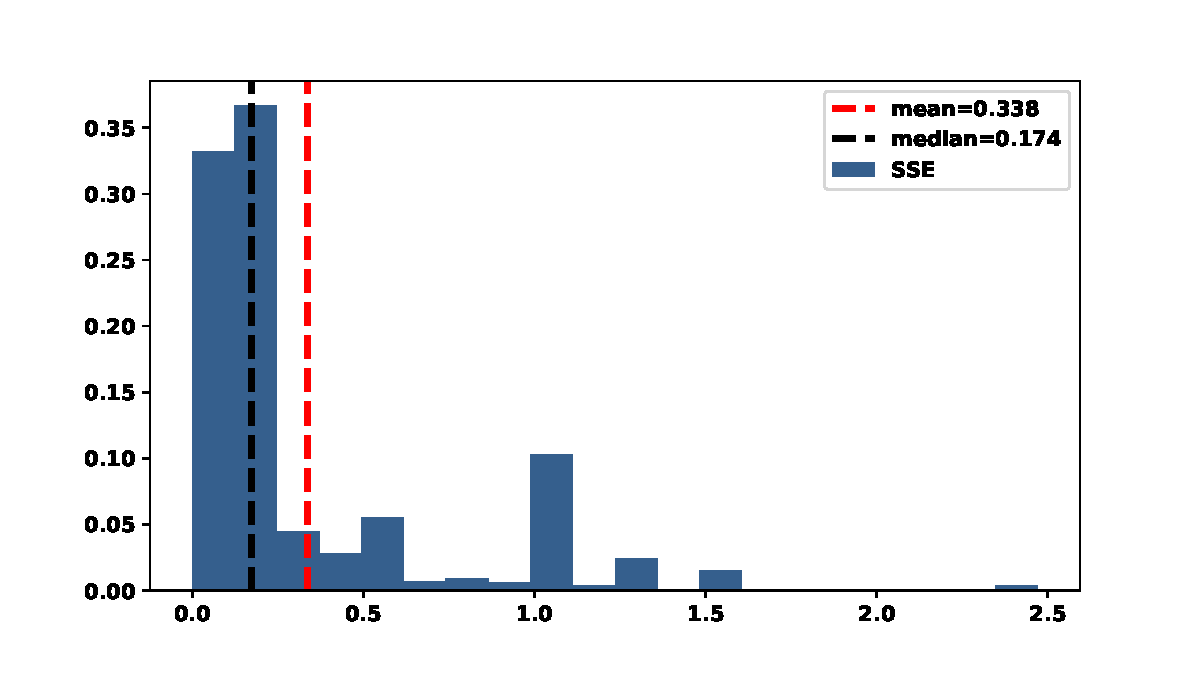
\includegraphics[width=\linewidth]{src/chapters/05/paper/Memory-size-in-the-prisoners-dilemma/img/best_respones_sserror.pdf}
            \end{center}
                \caption{Distribution of SSE for memory-one best responses, when \(N=2\).}
                \label{fig:sserror_mem_one}
    \end{minipage}\hspace{1cm}
    \begin{minipage}{0.25\textwidth}
        \centering
        \captionsetup{type=table}
        \resizebox{.75\columnwidth}{!}{%
            \begin{tabular}{lr}
\toprule
{} &     SSE \\
\midrule
count  &  1000.00000 \\
mean   &     0.33762 \\
std    &     0.39667 \\
min    &     0.00000 \\
5\%     &     0.02078 \\
25\%    &     0.07597 \\
50\%    &     0.17407 \\
95\%    &     1.05943 \\
max    &     2.47059 \\
median &     0.17407 \\
skew   &     1.87231 \\
kurt   &     3.60029 \\
\bottomrule
\end{tabular}
}
            \caption{Summary statistics SSE of best response memory one strategies included
            tournaments of \(N=2\).}
            \label{table:sserror_stats}
      \end{minipage}
\end{figure}

\subsection{Memory-one best responses in evolutionary dynamics}\label{subsection:best_respnse_evolutionary_setting}

As mentioned in section~\ref{section:utility}, the IPD is commonly studied in
Moran processes, and generally, in evolutionary processes. In these settings self
interactions are key. This section extends the formulation of best responses
in evolutionary dynamics, more specifically, the optimisation problem of
(\ref{eq:mo_tournament_optimisation}) is extended to
include self interactions.

Self interactions can be incorporated in the formulation
that has been used so far. The utility is given by,

\begin{equation}
    \frac{1}{N} \sum\limits_{i=1} ^ {N} {u_q}^{(i)} (p) + u_p(p)
\end{equation}

and the optimisation problem of (\ref{eq:mo_tournament_optimisation}) is modified to give:

\begin{equation}\label{eq:mo_evolutionary_optimisation}
    \begin{aligned}
    \max_p: & \ \frac{1}{N} \sum\limits_{i=1} ^ {N} {u_q}^{(i)} (p) + u_p(p)
    \\
    \text{such that}: & \ p \in \R_{[0, 1]}
    \end{aligned}
\end{equation}

For determining the memory-one best response in an evolutionary setting,
an algorithmic approach is considered, called \textit{best
response dynamics}. Best response dynamics are commonly used in evolutionary
game theory. They represent a class of strategy updating rules, where players in
the next round are determined by their best responses to some subset of the
population. The best response dynamics approach used in this manuscript is given by
Algorithm~\ref{algo:best_response_dynamics}.

% \begin{minipage}{.6\textwidth}
    \begin{algorithm}[H]
        $p^{(t)}\leftarrow (1, 1, 1, 1)$\;
        \While{$p^{(t)} \neq p ^{(t -1)}$}{
         $p^{(t + 1)} =  \text{argmax} \frac{1}{N} \sum\limits_{i=1} ^ {N} u_{q^{(i)}}
         (p^{(t)}) + u_{p^{(t)}}(p^{(t)})$\;
        }
        \caption{Best response dynamics Algorithm}
        \label{algo:best_response_dynamics}
    \end{algorithm}
% \end{minipage}

The best response dynamics algorithm starts by setting an initial
solution \(p^{(1)}=(1, 1, 1, 1)\), and repeatedly finds a strategy that maximises
(\ref{eq:mo_evolutionary_optimisation}) using Bayesian optimisation. The
algorithm stops once a cycle (a sequence of iterated evaluated points) is
detected. A numerical example of the algorithm is given in Figure~\ref{fig:best_response_dynamics_results}.

\begin{figure}[!htbp]
    \centering
    \includegraphics[width=.6\textwidth]{src/chapters/05/paper/Memory-size-in-the-prisoners-dilemma/img/best_response_dynamics_example.pdf}
    \caption{Best response dynamics with \(N=2\). More specifically, for
    \(q ^{(1)}=(\frac{59}{250},
                \frac{1031}{10000},
                \frac{99}{250},
                \frac{1549}{10000})\) and
    \(q ^{(2)}=(\frac{133}{2000},
                \frac{803}{2000},
                \frac{9179}{10000},
                \frac{2001}{2500})\).}
\label{fig:best_response_dynamics_results}
\end{figure}

The algorithm has been used to estimate the best response in an evolutionary
setting for each of the 1000 pairs of opponents described in
section~\ref{subsection:best_response_n_2}. These are also included in the data
set~\cite{glynatsi2019}, and moreover, the SSE method has also been applied. The
distribution of SSE is given by Figure~\ref{fig:sserror_mem_one} and a
statistical summary by Table~\ref{table:sserror_stats}.

\begin{figure}[!htbp]
    \begin{minipage}{0.65\textwidth}
            \begin{center}
            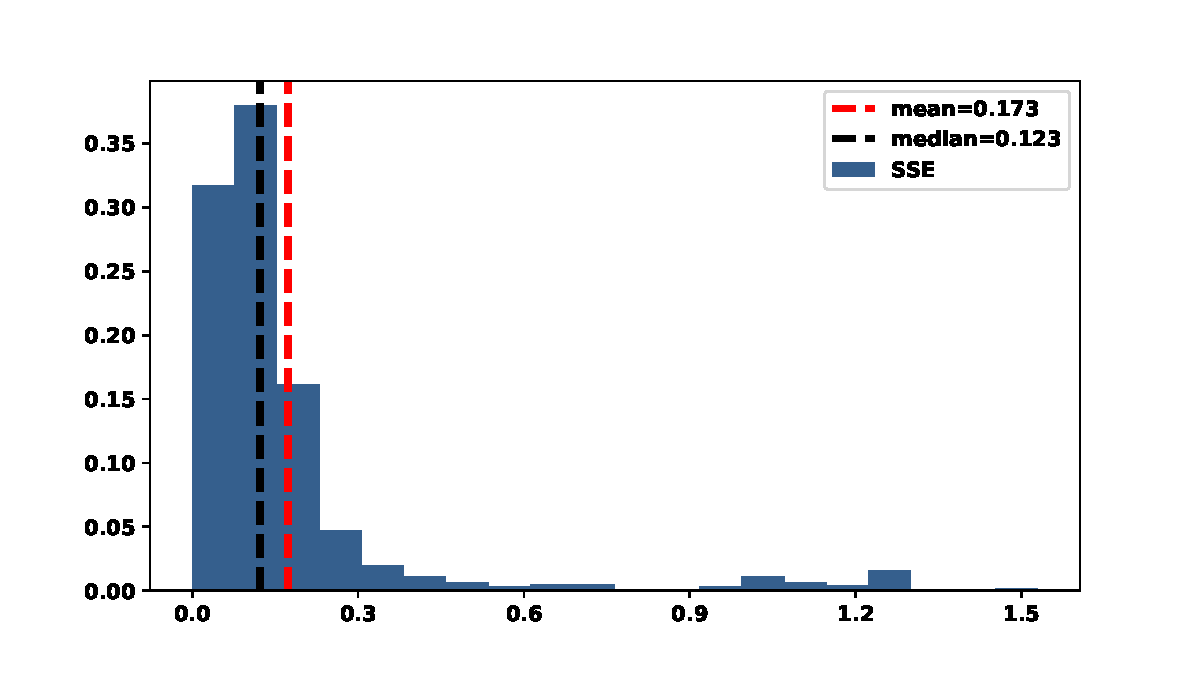
\includegraphics[width=\linewidth]{src/chapters/05/paper/Memory-size-in-the-prisoners-dilemma/img/evo_sserror.pdf}
            \end{center}
            \caption{Distribution of SSE of best response memory-one strategies in
            evolutionary settings, when \(N=2\).}
            \label{fig:sserror_mem_one}
    \end{minipage}\hspace{1cm}
    \begin{minipage}{0.25\textwidth}
        \centering
        \captionsetup{type=table}
        \resizebox{.75\columnwidth}{!}{%
            \begin{tabular}{lr}
\toprule
{} &  SSE \\
\midrule
count  &    1000.00000 \\
mean   &       0.17326 \\
std    &       0.23489 \\
min    &       0.00001 \\
5\%     &       0.01497 \\
25\%    &       0.05882 \\
50\%    &       0.12253 \\
95\%    &       0.67429 \\
max    &       1.52941 \\
median &       0.12253 \\
skew   &       3.41839 \\
kurt   &      11.92339 \\
\bottomrule
\end{tabular}
}
            \caption{Summary statistics SSE of best response memory-one strategies in
            evolutionary settings, when when \(N=2\).}
            \label{table:sserror_stats}
      \end{minipage}
\end{figure}

Similarly to the results of section~\ref{subsection:best_response_n_2}, the
evolutionary best response strategy does not behave uniformly extortionately. A
larger value of both the kurtosis and the skewness of the SSE distribution
indicates that in evolutionary settings a memory-one best response is even more
adaptable.

The difference between best responses in tournaments and in evolutionary
settings is further explored by Fig.~\ref{fig:behaviour_violin_plots}.
Though, no statistically significant differences have been found, from
Fig.~\ref{fig:behaviour_violin_plots}, it seems that evolutionary best
response has a higher median $p_2$; which corresponds to the probability of cooperating
after receiving a defection. Thus, they are more likely to forgive after
being tricked. This is due to the fact that they could be playing against
themselves, and they need to be able to forgive so that future cooperation can
occur.

\begin{figure}[!htbp]
    \centering
    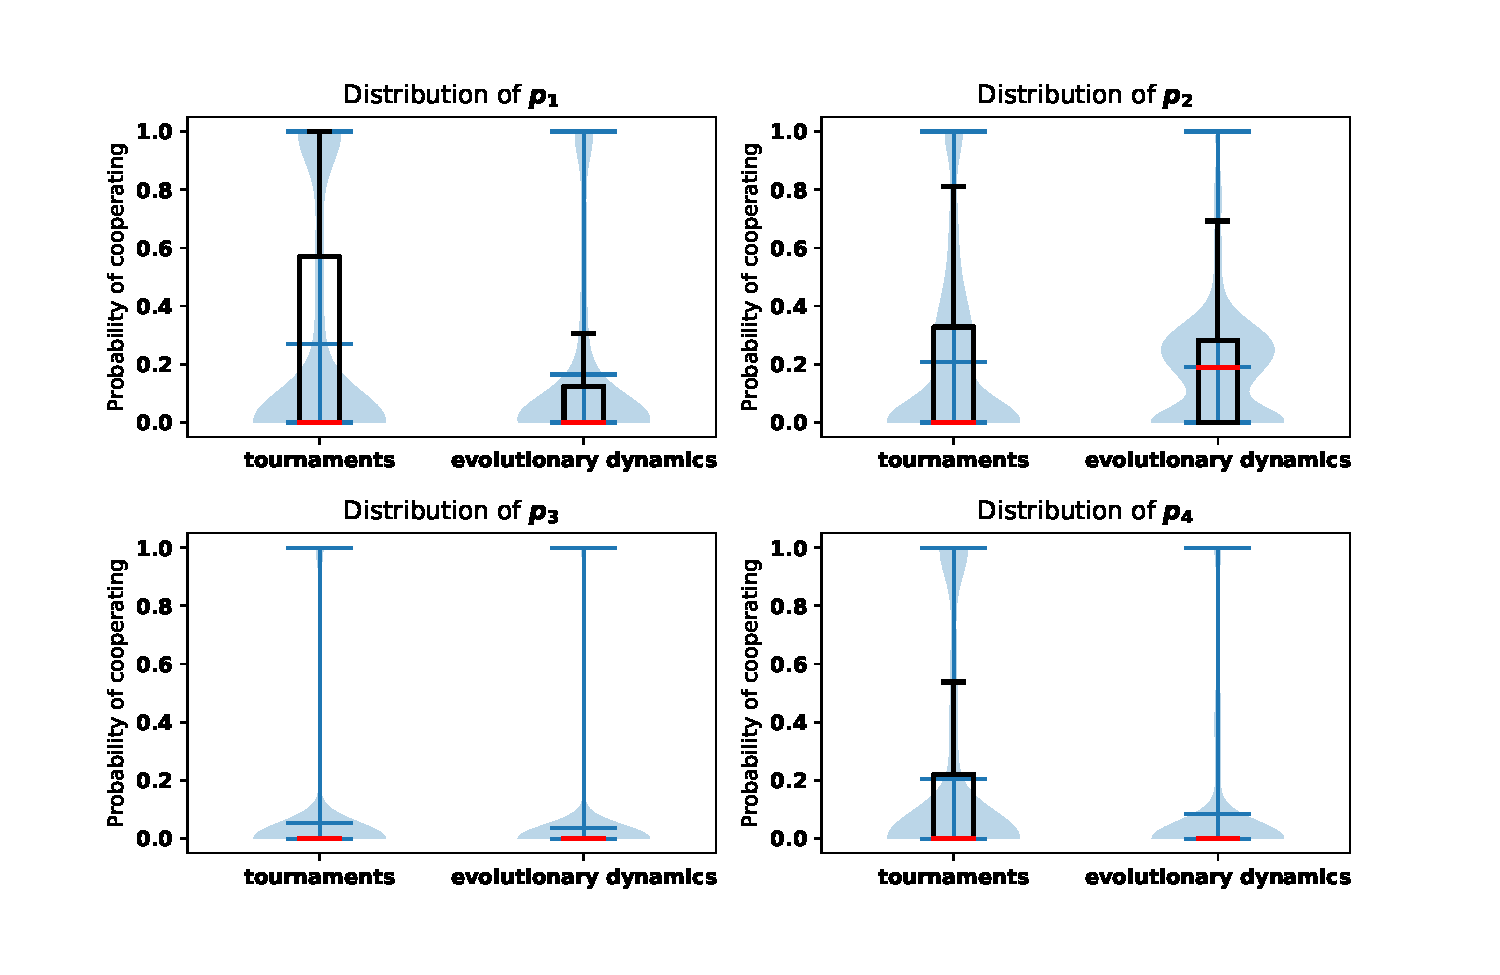
\includegraphics[width=.8\textwidth]{src/chapters/05/paper/Memory-size-in-the-prisoners-dilemma/img/behaviour_violin_plots.pdf}
    \caption{Distributions of \(p^*\) for both best response and evolutionary memory-one
    strategies.}
    \label{fig:behaviour_violin_plots}
\end{figure}

\begin{table}[!htbp]
    \centering
    \resizebox{.7\columnwidth}{!}{%
    \begin{tabular}{lrrr}
\toprule
                   &  tournaments' median &  evolutionary dynamics' median &  p\-values \\
\midrule
Distribution $p_1$ &         0.000 &               0.000 &       0.0 \\
Distribution $p_2$ &         0.000 &               0.189 &       0.0 \\
Distribution $p_3$ &         0.000 &               0.000 &       0.0 \\
Distribution $p_4$ &         0.000 &               0.000 &       0.0 \\
\bottomrule
\end{tabular}
}
    \caption{A non parametric test, Wilcoxon Rank Sum, has been performed to
    tests the difference in the median values of the cooperation probabilities
    in tournaments versus evolutionary settings. A non parametric test is used because
    is evident that the data are skewed.}\label{table:wilcoxon_tests}
\end{table}

\subsection{Longer memory best response}\label{subsection:longer_memory_best_response}

This section focuses on the memory size of strategies. The effectiveness of
memory in the IPD has been previously explored in the literature, as
discussed in section~\ref{section:introduction}, however, none of the
previous works has compared the performance of longer-memory strategies to
memory-one best responses.

The strategy used in this Chapter is one of the archetypes described in Chapter
\ref{chapter:literature_review} called \textit{Gambler} introduced
in~\cite{Harper2017}. As a reminder, Gambler is a stochastic version of a lookup
table. It makes probabilistic decisions based on the opponent's \(n_1\) first
moves, the opponent's \(m_1\) last moves and the player's \(m_2\) last moves was
introduced. In this Chapter Gambler with parameters: $n_1 = 2, m_1 = 1$ and $m_2
= 1$ is used as a longer-memory strategy.

By considering the opponent's first two moves, the opponents last move and the
player's last move, there are only 16 $(4 \times 2 \times 2)$ possible outcomes
that can occur, furthermore, Gambler also makes a probabilistic decision of
cooperating in the opening move. Thus, Gambler is a function \(f: \{\text{C,
D}\} \rightarrow [0, 1]_{\R}\). This can be hard coded as an element
of \([0, 1]_{\R} ^ {16 + 1}\), one probability for each outcome plus the opening
move. Hence, compared to (\ref{eq:mo_tournament_optimisation}), finding an
optimal Gambler is a 17 dimensional problem given by:

\begin{equation}\label{eq:gambler_optimisation}
    \begin{aligned}
    \max_p: & \ \sum_{i=1} ^ {N} {U_q}^{(i)} (f)
    \\
    \text{such that}: & \ f \in \R_{[0, 1]}^{17}
    \end{aligned}
\end{equation}

Note that (\ref{eq:tournament_utility}) can not be used here for the utility
of Gambler, and actual simulated players are used. This is done using~\cite{axelrodproject}
with 500 turns and 200 repetitions, moreover, (\ref{eq:gambler_optimisation})
is solved numerically using Bayesian optimisation.

Similarly to previous sections, a large data set has been generated with
instances of an optimal Gambler and a memory-one best response, available
at~\cite{glynatsi2019}. Estimating a best response Gambler (17 dimensions) is
computational more expensive compared to a best response memory-one (4
dimensions). As a result, the analysis of this section is based on a total of
130 trials. For each trial two random opponents have been selected. The 130 pair
of opponents are a sub set of the opponents used in
section~\ref{subsection:best_response_n_2}-
\ref{subsection:best_respnse_evolutionary_setting}. The distributions of their
transition probabilities are given in Figures
\ref{fig:first_opponents_probabilities_with_gambler} and
\ref{fig:first_opponents_probabilities_with_gambler}.

\begin{figure}[!htbp]
    \begin{subfigure}{0.49\textwidth}
        \centering
        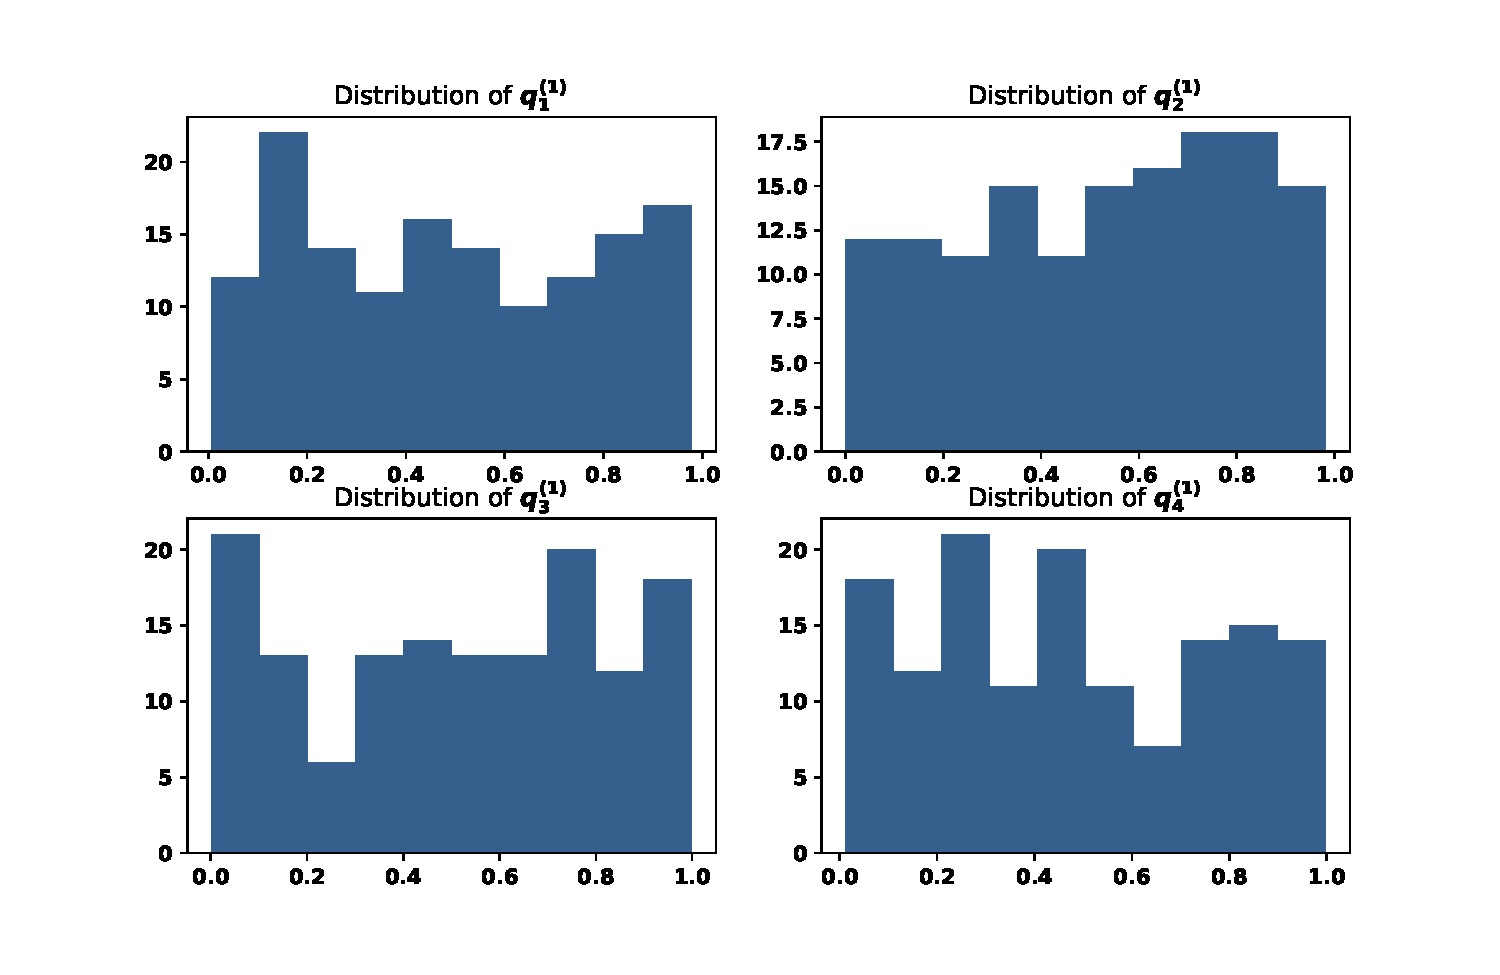
\includegraphics[width=\linewidth]{src/chapters/05/paper/Memory-size-in-the-prisoners-dilemma/img/first_opponent_probabilities_with_gambler.pdf}
        \subcaption{Distributions of first opponents' probabilities for longer memory experiment.}
        \label{fig:first_opponents_probabilities_with_gambler}
    \end{subfigure}
    \begin{subfigure}{0.49\textwidth}
        \centering
        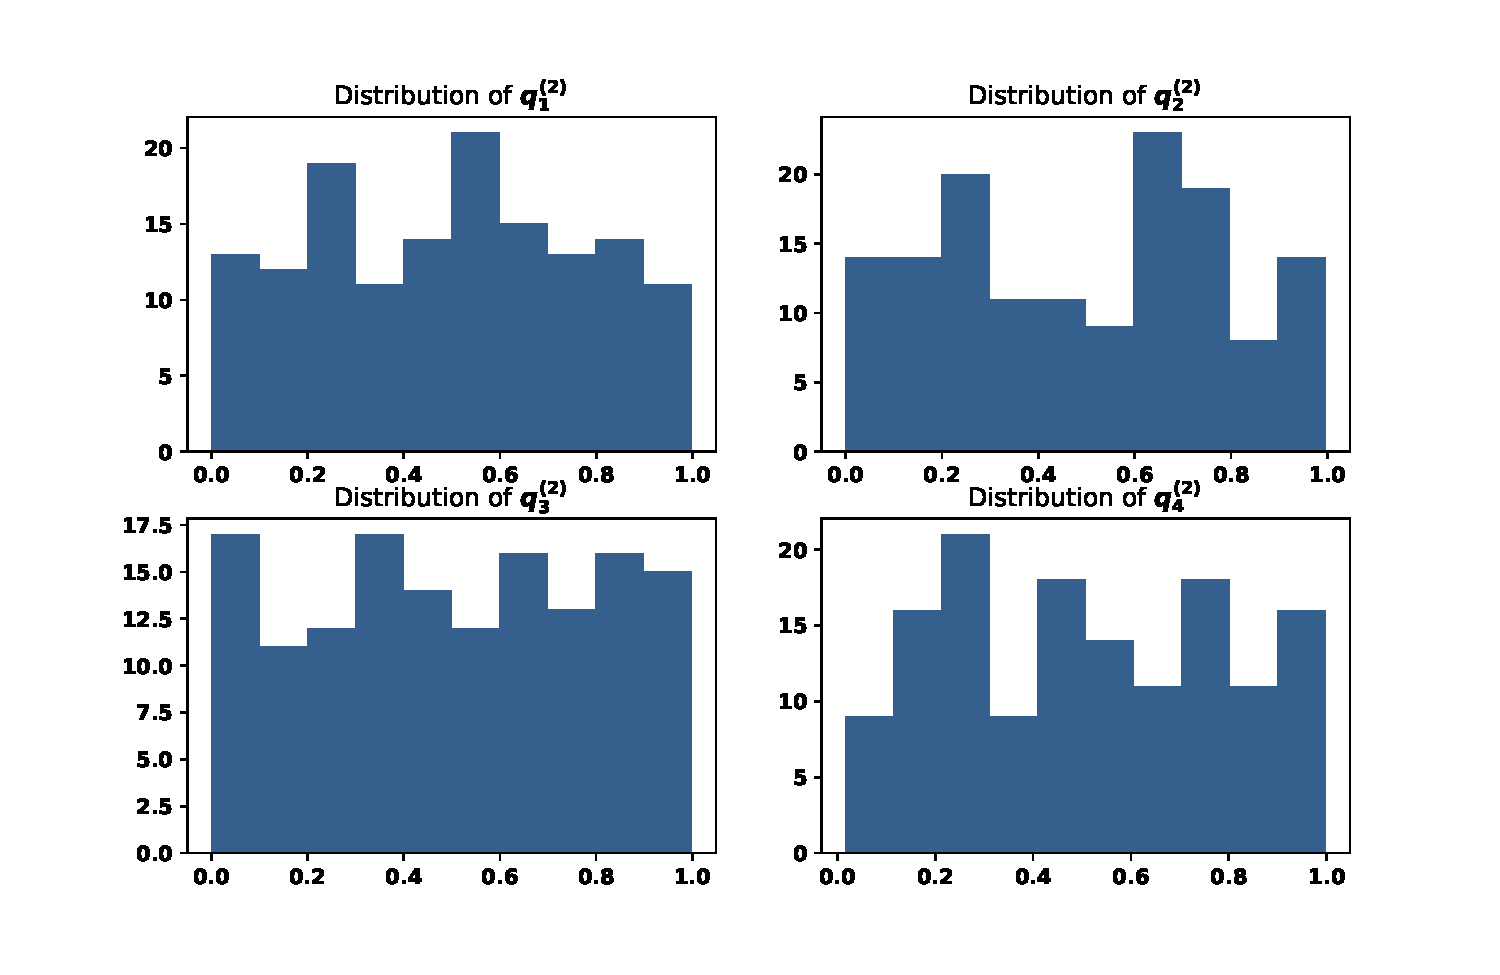
\includegraphics[width=\linewidth]{src/chapters/05/paper/Memory-size-in-the-prisoners-dilemma/img/second_opponent_probabilities_with_gambler.pdf}
        \subcaption{Distributions of second opponents' probabilities for longer memory experiment.}
        \label{fig:second_opponents_probabilities_with_gambler}
    \end{subfigure}
\end{figure}

The ratio between Gambler's utility and the best response memory-one strategy's utility has been calculated and its distribution in
given in Fig.~\ref{fig:utilities_gambler_mem_one}.
It is evident from Fig.~\ref{fig:utilities_gambler_mem_one} that
Gambler always performs as well as the best response memory-one strategy and often performs better. There are
no points where the ratio value is less than 1, thus Gambler never performed less
than the best response memory-one strategy and in places outperforms it. This seems to be at odd with the
result of~\cite{Press2012} that against a memory-one opponent having a longer memory
will not give a strategy any
advantage. However, against two memory-one opponents Gambler's performance is better than
the optimal memory-one strategy. This is evidence that in the case of two opponents having a
shorter memory is limiting.

\begin{figure}[!htbp]
    \centering
    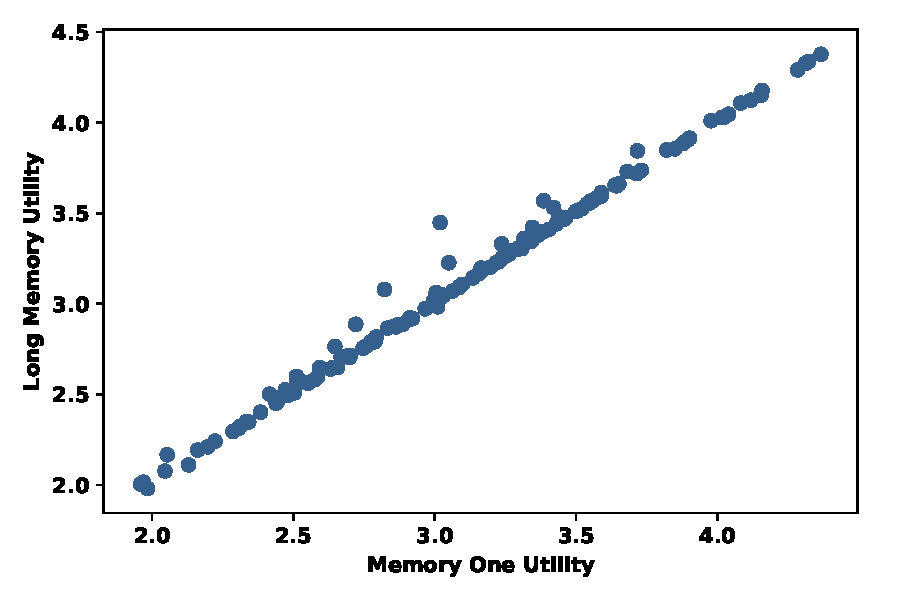
\includegraphics[width=.55\textwidth]{src/chapters/05/paper/Memory-size-in-the-prisoners-dilemma/img/gambler_performance_against_mem_one.pdf}
    \caption{Utilities of Gambler and best response memory-one strategies for
    130 different pair of opponents.}\label{fig:utilities_gambler_mem_one}
\end{figure}

\section{Stability of defection}\label{section:stability_of_defection}

An immediate result from the formulation used so far in this Chapter can be
obtained by evaluating the sign of Equation (\ref{eq:tournament_utility})'s derivative
at \(p=(0, 0, 0, 0)\). If at that point the
derivative is negative, then the utility of a player only decreases if they were
to change their behaviour, and thus defection at that point is stable.

\begin{lemma}\label{lemma:stability_of_defection}
    In a tournament of \(N\) players \(\{q^{(1)}, q^{(2)}, \dots, q^{(N)} \}\)
    for \(q^{(i)} \in \R_{[0, 1]} ^ 4\)
    defection is stable if the transition probabilities of the
    opponents satisfy conditions Equation \ref{eq:defection_condition_one} and Equation (\ref{eq:defection_condition_two}).

    \begin{equation}\label{eq:defection_condition_one}
        \sum_{i=1} ^ N (c^{(i)T} \bar{a}^{(i)} - \bar{c}^{(i)T} a^{(i)}) \leq 0
    \end{equation}

    while,

    \begin{equation}\label{eq:defection_condition_two}
        \sum_{i=1} ^ N \bar{a}^{(i)} \neq 0
    \end{equation}
\end{lemma}

\begin{proof}
    For defection to be stable the derivative of the utility
    at the point \(p = (0, 0, 0, 0)\) must be negative.

    Substituting \(p = (0, 0, 0, 0)\) in
    Equation (\ref{eq:mo_tournament_derivative}) gives:

    \begin{equation}
        \left.\frac{d\sum\limits_{i=1} ^ {N} {u_q}^{(i)} (p)}{dp} \right\rvert_{p=(0,0,0,0)} =
    \sum_{i=1} ^ N \frac{(c^{(i)T} \bar{a}^{(i)} - \bar{c}^{(i)T} a^{(i)})}
    {(\bar{a}^{(i)})^2}
    \end{equation}

    The sign of the numerator \( \displaystyle\sum_{i=1} ^ N (c^{(i)T} \bar{a}^{(i)} - \bar{c}^{(i)T} a^{(i)})\)
    can vary based on the transition probabilities of the opponents.
    The denominator can not be negative, and otherwise is always positive.
    Thus the sign of the derivative is negative if and only if
    \( \displaystyle\sum_{i=1} ^ N (c^{(i)T} \bar{a}^{(i)} - \bar{c}^{(i)T} a^{(i)}) \leq 0\).
\end{proof}

Consider a population for which defection is known to be stable. In that
population all the members will over time adopt the same behaviour; thus in such
population cooperation will never take over. This is demonstrated in
Figure~\ref{fig:stability_of_defection}.
These have been simulated using~\cite{axelrodproject} an open
source research framework for the study of the IPD.

\begin{figure}[!htbp]
    \centering
    \includegraphics[width=.4\linewidth]{src/chapters/05/paper/Memory-size-in-the-prisoners-dilemma/img/stability_of_defection_plots.pdf}
    \caption{A. For \(q_{1}=(0.22199, 0.87073, 0.20672, 0.91861)\),
    $q_{2}=(0.48841, 0.61174, 0.76591, 0.51842)$ and
    $q_{3}=(0.2968, 0.18772, 0.08074, 0.73844)$, Equation~\ref{eq:defection_condition_one} and
    Equation~\ref{eq:defection_condition_two} hold and Defector takes over the
    population. B. For $q_{1}=(0.96703, 0.54723, 0.97268, 0.71482)$,
    $q_{2}=(0.69773, 0.21609, 0.97627, 0.0062)$ and
    $q_{3}=(0.25298, 0.43479, 0.77938, 0.19769)$, Equation~\ref{eq:defection_condition_one} fails
    and Defector does not take over the population.}\label{fig:stability_of_defection}
\end{figure}

\section{Chapter Summary}

This Chapter has considered best response strategies in the IPD game, and
more specifically, memory-one best responses. It has proven that there is
a compact way of identifying a memory-one best response to a group of opponents,
and moreover, that there exists a condition for which in an
environment of memory-one opponents defection is the stable choice.
The later parts of this paper focused on a series of empirical results, where it
was shown that the performance and the evolutionary stability of memory-one
strategies rely not on extortion but on adaptability. Finally, it was shown that
memory-one strategies' performance is limited by their memory in cases where
they interact with multiple opponents.

Following the work described in~\cite{Nowak1989}, where it was shown that the
utility between two memory-one strategies can be estimated by a Markov
stationary state, we proved that the utilities can be written as a ration of two
quadratic forms in $R^4$, Theorem~\ref{theorem:quadratic_form_u}. This was
extended to include multiple opponents, as the IPD is commonly studied in such
situations, Theorem~\ref{theorem:tournament_utility}.
The formulation of Theorem~\ref{theorem:tournament_utility} allowed us to introduce an approach for identifying
memory-one best responses to any number of opponents;
Lemma~\ref{lemma:memone_group_best_response}. This does not only have game
theoretic novelty, but also a mathematical novelty of solving quadratic ratio
optimisation problem where the quadratics are non concave. The results of
Lemma~\ref{lemma:memone_group_best_response} were also used to define a
condition for which defection is known to be stable.

Several experimental results were presented in this Chapter. These results were mainly to
investigate the behaviour of memory-one strategies and their limitations. In
Sections~\ref{subsection:best_response_n_2}
and~\ref{subsection:best_respnse_evolutionary_setting}, a large data set which
contained best responses in tournaments and in evolutionary settings for $N=2$
was generated. This allowed us to investigate their respective behaviours, and
whether it was extortionate acts that made them the most favourable strategies.
However, it was shown that it was not extortion but adaptability that allowed
the strategies to gain the most from their interactions.
In evolutionary settings it was specifically shown that being adaptable and being
able to forgive after being tricked were key factors. In section~\ref{subsection:longer_memory_best_response}, the performance of
memory-one strategies was put against the performance of a longer memory
strategy called Gambler. There were several cases where Gambler would outperform
the memory-one strategy, however, a memory-one strategy never managed to outperform
a Gambler. This result occurred whilst considering a Gambler with a sufficiently
larger memory but not a sufficiently larger amount of information regarding
the game.
